\documentclass{article}
\usepackage[utf8]{inputenc}
\usepackage[brazilian]{babel}
\usepackage[utf8]{inputenc}
\usepackage[T1]{fontenc}
\usepackage{tikz}
\usepackage{natbib}
\usepackage{graphicx}
\usepackage{hyperref}
\usepackage{makeidx}
\usepackage{xcolor}
\usepackage{listings}
\usepackage{tikz}
\usepackage{verbatim}

\begin{document}

    \begin{titlepage} %iniciando a "capa"
        \begin{center} %centralizar o texto abaixo
            {\large Universidade Federal de Uberlândia}\\[0.2cm] %0,2cm é a distância entre o texto dessa linha e o texto da próxima
            {\large Ciência da Computaçõa}\\[0.2cm]
            {\large Construção de Compiladores}\\[5.1cm]
            {\bf \huge Construção do mini compilador Python para CLR}\\[5.1cm] % o comando \bf deixa o texto entre chaves em negrito. O comando \huge deixa o texto enorme
        \end{center} %término do comando centralizar
            
            {\large Aluno: Arthur Xavier Giffoni}\\[0.2cm] % o comando \large deixa o texto grande
            {\large E-mail: arthurxaviergiffoni@gmail.com}\\[0.3cm]
            {\large Professor:Alexsandro Santos Soares}\\[3.1cm]
            
        \begin{center}
            {\large Abril, 2017}\\
        \end{center}
    \end{titlepage} %término da "capa"


\renewcommand*\contentsname{Sumário}

% Definindo novas cores
\definecolor{verde}{rgb}{0.25,0.5,0.35}
\definecolor{jpurple}{rgb}{0.5,0,0.35}
% Configurando layout para mostrar codigos Java

\lstset{
  language=Java,
  basicstyle=\ttfamily\small, 
  keywordstyle=\color{jpurple}\bfseries,
  stringstyle=\color{red},
  commentstyle=\color{verde},
  morecomment=[s][\color{blue}]{/**}{*/},
  extendedchars=true, 
  showspaces=false, 
  showstringspaces=false, 
  numbers=left,
  numberstyle=\tiny,
  breaklines=true, 
  backgroundcolor=\color{cyan!10}, 
  breakautoindent=true, 
  captionpos=b,
  xleftmargin=0pt,
  tabsize=4
}
\pagestyle{empty}

%\begin{document}

\tableofcontents
\newpage

%%%%%%%%%%%%%%%%%%%%%%%%%%%%%%%%%%%%%%%%%%%%%%%%%%%%%%%%%%%%%%%%%%%%%%%%%%%

\section{Introdução}
Common Language Runtime - CLR, é um ambiente de tempo de execução do .NET Framework, o qual que executa o código e provê serviços que tornam o processo de desenvolvimento mais fácil.Compiladores e ferramentas expõem as funcionalidades do Common Language Runtime e habilitam você escrever código que se beneficia desse ambiente de execução gerenciado. Código que você desenvolve com um compilador de linguagem que tem como alvo o runtime é chamado de código gerenciado; ele se beneficia de recursos como integração entre linguagens, tratamento de exceção entre linguagens, segurança aprimorada, suporte a versionamento e implantação, um modelo simplificado para interação entre componentes, e serviços de depuração e de perfil.

O CLR descreve o código executável e o ambiente de execução que formam
o núcleo do Framework .NET da Microsoft, do MONO e do Portable.NET. A Common Language Runtime é uma máquina virtual que segue um padrão
internacional e a base para a criação e execução de ambientes de desenvolvi-
mento em que as linguagens e as bibliotecas trabalham juntos.

Programas em linguagem Visual Basic, Visual C ++ ou C \# são compilados em um formulário intermediário de codificar chamado Common Intermediate Language (CIL) em um arquivo de execução portátil (PE) que pode, em seguida, ser gerenciado e executado pelo Common Language Runtime.

%%%%%%%%%%%%%%%%%%%%%%%%%%%%%%%%%%%%%%%%%%%%%%%%%%%%%%%%%%%%%%%%%%%%%%%%%%%
\section{Arquitetura}

O common language runtime (CLR) API de depuração foi projetado para ser usado como se fosse parte do kernel do sistema operacional. Em código não gerenciado, quando um programa gera uma exceção, o kernel suspende a execução do processo e passa as informações de exceção para o depurador usando o Win32 API de depuração. API de depuração CLR fornece a mesma funcionalidade para código gerenciado. Quando o código gerenciado gera uma exceção, a API de depuração CLR suspende a execução do processo e passa as informações de exceção para o depurador.


API de depuração CLR inclui dois componentes principais:

\begin{itemize}
    
\item A DLL de depuração, que é sempre carregada no mesmo processo como o programa que está sendo depurado. O controlador de tempo de execução é responsável pela comunicação com o CLR e executar o controle de execução e inspeção de threads que estejam executando o código gerenciado.

\item A interface do depurador, que é carregada em um processo diferente do programa que está sendo depurado. A interface do depurador é responsável pela comunicação com o controlador de tempo de execução em nome do depurador. Também é responsável pela manipulação de eventos de depuração do Win32 que vêm do processo que está sendo depurado e ambos lidando com esses eventos ou passá-los para um depurador de código não gerenciado. A interface do depurador é a única parte da API que tem uma API exposta de depuração CLR.
\end{itemize}
O CLR API de depuração não oferece suporte ao uso remoto entre computadores ou entre processos; ou seja, um depurador que usa a API deverá fazê-lo de dentro de seu próprio processo, conforme a figura no seguinte diagrama de arquitetura da API. Esta ilustração mostra onde os diferentes componentes do CLR API de depuração estão localizados e como eles interagem com o CLR e o depurador.

\begin{center}
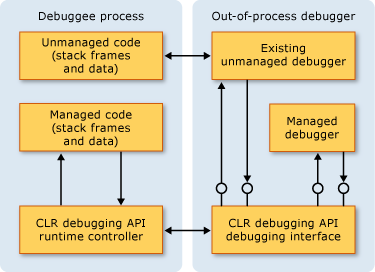
\includegraphics[scale=0.7]{ArquiteturaCLR.png}
\end{center}

%%%%%%%%%%%%%%%%%%%%%%%%%%%%%%%%%%%%%%%%%%%%%%%%%%%%%%%%%%%%%%%%%%%%%%%%%%
\section{Instruções}
O assembly da plataforma, MSIL, é um conjunto de instruções baseado em
pilha e orientado a objetos. As funcionalidade de algumas intruções em relação a manipulação da pilha listadas a seguir:

\begin{itemize}
\item add: retira os dois elementos do topo da pilha e coloca o resultado no
topo.
\item add.ovf: mesma operação que o add porém com uma verificação de
overflow(gerando uma exceção de overflow).
\item and: retira os dois elementos do topo da pilha, faz a operação and bit
a bit e coloca o resultado no topo da pilha.
\item arglist: pega argumento da lista (usado em para pegar argumentos de
função)
\item beq.[length]: branch para label se o dois valores da pilha são iguais
\item bge.[length]: branch para label se o primeiro valor é menor que o se-
gundo da pilha
\item bge.un.[length]: branch para label se maior ou igual, comparação sem
sinal
\item bgt.[length]: branch para label quando o segundo valor é maior que o
primeiro
\item bgt.un.[length]: branch para label quando o topo é maior que o segundo
valor, sem sinal
\item ble.[length]: branch para label quando o topo é menor ou igual ao
segundo valor
\item ble.un.[length]: branch para label se topo é menor ou igual ao segundo
valor, sem sinal
\item blt.[length]: branch para label quando quando o topo é menor que o
segundo valor
\item blt.un.[length]: branch para label se topo é menor que segundo valor,
sem sinal
\item bne.un[length]: branch para label quando topo não for igual ou não
ordenada
\item br.[length]: branch incondicional
\item break: instrução breakpoint
\item brfalse.[length]: branch para label se falso, nulo, ou zero
\item brtrue.[length]: branch para label quando não falseo ou não nulo
\item call: chama um método
\item calli: chama um método indireto
\item ceq: compara se igual
\item cgt: compara se maior que
\item cgt.un: compara maior que,sem sinal e não ordenado
\item ckfinite: Checa se é um número real e finito
\item clt: compara se menor que
\item clt.un: compara se menor que, sem sinal e não ordenado
\item conv.[to type]: conversão de dados
\item conv.ovf.[to type]: conversão de dados com detecção de overflow
\item conv.ovf.[to type].un: conversão de dados sem sinal com detecção de
overflow
\item cpblk: copia dados da memória para a memória
\item div: divide valores
\item div.un: divide valores inteiros, sem sinal
\item dup: duplica o valor do topo da pilha
\item endfilter: fim do filtro da cláusula de SEH
\item endfinally: finaliza a cláusula do bloco de exceção
\item initblk: inciliaza um bloco de memória para um valores
\item jmp: pula para um método
\item jmpi: pula para um ponteiro de método
\item ldarg.[length]: carrega um argumento na pilha
\item ldarga.[length]: carrega um argumento a partir de um endereço
\item ldc.[type]: carrega uma constante numérica
\item ldftn : carrega um ponteiro de método
\item ldind.[type]: carrega um valor indireto na pilha
\item ldloc: load local variable onto the stack
\item ldloc: carrega na pilha o valor da variavel local.
\item ldloca index: carrega na pilha o valor da variavel local com index.
\item ldnull: carrega na pilha um ponteiro pra null
\item leave target: sai de uma região protegida do códdigo
\item localloc: aloca um espaço na memory pool do tamanho do primeiro
elemento dap ilha e retorna o endereço da área.
\item mul: multiplica os dois valores do topo da pilha(retirando-os) e coloca
o resultado.
\item mul.ovf.[type]: multiplica valores inteiros levando em conta o overflow.
\item neg: retira o valor do topo da pilha, nega ele e põe o resultado no topo,
retornando o mesmo tipo de operando.
\item nop: faz nada :D
\item not: retira um inteiro e coloca seu complemento(inverção de bits) na
pilha.
\item or: faz o OU bit a bit dos dois valores inteiros no topo da pilha(retirando-
os) e coloca o resultado.
\item pop: remove o elemento do topo da pilha.
\item rem: computa o resto da divisão do valor abaixo do topo da pilha pelo
valor que está no topo(retirando-os) e coloca o resultado no topo.
\item rem.un: mesmo que o rem só que para inteiros unsigned.
\item ret: retorna para o método corrente, o tipo de retorno do método em
questão será o utilizado.
\item shl: Deslocamento de inteiro para a esquerda...,
valor, qntd d e d eslocamentoretiraestesdoisdapilhaecolocaoresultado.
\item shr: mesmo que o shl porém com deslocamneto para a direita.
\item shr.un: memso que shr só que para inteiros unsigned.
\item starg.[length]: retira o elemento do topo da pilha e o coloca em um
argumento(starg num).
\item stind.[type]: coloca o valor(topo da pilha) no endereço (logo abaixo).
\item stloc: retira o valor do topo da pilha e o poe na variavel(stloc x)
\item sub: subtrai do segundo valor o primeiro e poe o resultado no topo.
\item sub.ovf.[type]: subtração de inteiros com overflow
\item tail.: deve preceder imediatamente instruções de call, calli ou callvirt.
Ela indica que o método corrente na pilha deve ser removido antes da
chamada da função ser executada.
\item unaligned. (prefix code): expecifica que o endereço na pilha não está
alinhado ao tamanho natural.
\item volatile. (prefix code): especifica que o endereço no topo da pilha é
volátil.
\item xor: executa a operação XOR(bit a bit) entre os dois primeiros elemen-
tos da pilha colocando seu resultado na mesma.
\item ldelem.[type]: carrega um elemento do vetor(segunda posição) no in-
dex(primeira posição, topo da pilha) na pilha
\item ldelema: poe o endereço do vetor na posição index na pilha.
\item ldlen: poe na pilha o tamanho do vetor(topo da pilha)
\item ldstr: poe a string(ldstr string) no topo da pilha
\item newarr: cria um array com o tipo definido(newarr int32) onde seu ta-
manho está no topo da pilha.
\item sizeof: carrega o tamanho em bits do tipo definido(sizeof int32) na
pilha.
\item stelem.[type]: coloca no array(terceiro da pilha) no index(segunda da
pilha) o valor(topo da pilha).
\end{itemize}

%%%%%%%%%%%%%%%%%%%%%%%%%%%%%%%%%%%%%%%%%%%%%%%%%%%%%%%%%%%%%%%%%%%%%%%%%%%%%

\section{Instalações}
Nessa seção sera listados os comandos para instalação das ferramentas necessárias para manipulação e execução dos códigos. Antes de iniciar qualquer instalação no Linux, devemos atualizar nosso pacote utilizando o codigo:\\\

\fbox{\textbf{sudo apt-get update}}\\\\
Apos autualizado, podemos instalar as ferramentas especificas.


\subsection{Instalação do Mono}
Patrocinado pela Microsoft, Mono é uma implementação de código aberto do Microsoft .NET Framework baseado nos padrões ECMA para C \# e Common Language Runtime.
Para instalar o Mono com apt-get utiliza-se o pacote:\\

\fbox{\textbf{sudo apt-get install mono-complete}}\\\\


\subsection{Instalação do OCaml}
Para instalar o OCaml basta digitar o seguinte comando no terminal:\\

\fbox{\textbf{sudo apt-get install ocaml}}\\\\


\subsection{Instalação do Python}
Nesse trabalho iremos utilizar o Python 2.7. Para instalar basta digitar o seguinte comando no terminal:\\

\fbox{\textbf{sudo apt-get install python2.7}}\\\\

%%%%%%%%%%%%%%%%%%%%%%%%%%%%%%%%%%%%%%%%%%%%%%%%%%%%%%%%%%%%%%%%%%%%%%%%%%%%%

\section{Gerando a Tradução dos Programas}
Os programas em Python devem terminar com a Extensão ".py"\\

Para a transformação do codigo o mesmo deve ser convergido para C \# para depois ser lido o assembly. \\
Os programas em C \# devem terminar com a Extensão ".cs"\\

Executar o cógido Python \\

\fbox{\textbf{python nanoC.py}}\\\\

Compilar o cógido C \# e gerar o .exe\\

\fbox{\textbf{dmcs nanoC.cs}}\\\\


Gerar assembly em cima do oexecutavel C \# .exe \\

\fbox{\textbf{monodis nanoC.exe > nanoC.txt}}\\\\


\section{Códigos:  MiniPython - C\# - Assembly}

\subsection{nano01}

MiniPython nano01
\begin{lstlisting}
def nano01():
pass
\end{lstlisting}
MiniC\# nano01
\begin{lstlisting}
using System;

namespace nano01
{
	class Program
	{
		static void Main(String[] args){}
	}
}
\end{lstlisting}
Assembly nano01
\begin{lstlisting}
.assembly extern mscorlib{}

.assembly 'nano01'
{
  .ver  0:0:0:0
}
.module nano01.exe

.namespace nano01
{
  .class private auto ansi beforefieldinit Program
  	extends [mscorlib]System.Object
  {

    .method public hidebysig specialname rtspecialname 
           instance default void '.ctor' ()  cil managed 
    {
	    .maxstack 8
	    ldarg.0 
	    call instance void object::'.ctor'()
	    ret 
    } 

    // method line 2
    .method private static hidebysig 
            default void Main ()  cil managed 
    {
	    .entrypoint
	    .maxstack 0
	    ret 
    } 

  } 
}
\end{lstlisting}\\\\


%%%%%%%%%%%%%%%%%%%%%%%%%%%%%%%%%%%%%%%%%%%%%%%%%%%%%%%%%%%%%%


\subsection{nano02}

MiniPython nano02
\begin{lstlisting}
def nano02():
    n = int(n)
\end{lstlisting}

MiniC\# nano02
\begin{lstlisting}
using System;

namespace nano02
{
	class Program
	{
		static void Main(String[] args)
		{
			int n;
		}
	}
}
\end{lstlisting}

Assembly nano02
\begin{lstlisting}
.assembly extern mscorlib{}

.assembly 'nano02'
{
  .ver  0:0:0:0
}
.module nano02.exe

.namespace nano02
{
  .class private auto ansi beforefieldinit Program
  	extends [mscorlib]System.Object
  {

    .method public hidebysig specialname rtspecialname 
           instance default void '.ctor' ()  cil managed 
    {
	    .maxstack 8
	    ldarg.0 
	    call instance void object::'.ctor'()
	    ret 
    } 

    // method line 2
    .method private static hidebysig 
            default void Main ()  cil managed 
    {
	    .entrypoint
	    .maxstack 0
	    .locals init (int32	V_0)
	    ret 
    } 

  } 
}
\end{lstlisting}\\\\



%%%%%%%%%%%%%%%%%%%%%%%%%%%%%%%%%%%%%%%%%%%%%%%%%%%%%%%%%%%%%%





\subsection{nano03}

MiniPython nano03
\begin{lstlisting}
def nano03():
    n = int(n)
    n=1
\end{lstlisting}

MiniC\# nano03
\begin{lstlisting}
using System;

namespace nano03
{
	class Program
	{
		static void Main(String[] args)
		{
			int n;
			n = 1;
		}
	}

}
\end{lstlisting}

Assembly nano03
\begin{lstlisting}
.assembly extern mscorlib{}

.assembly 'nano03'
{
  .ver  0:0:0:0
}
.module nano03.exe

.namespace nano03
{
  .class private auto ansi beforefieldinit Program
  	extends [mscorlib]System.Object
  {

    .method public hidebysig specialname rtspecialname 
           instance default void '.ctor' ()  cil managed 
    {
	    .maxstack 8
	    ldarg.0 
	    call instance void object::'.ctor'()
	    ret 
    } 

    // method line 2
    .method private static hidebysig 
            default void Main ()  cil managed 
    {
	    .entrypoint
	    .maxstack 0
	    .locals init (int32	V_0)
	    ldc.i4.1
	    stloc.0
	    ret 
    } 

  } 
}
\end{lstlisting}\\\\

%%%%%%%%%%%%%%%%%%%%%%%%%%%%%%%%%%%%%%%%%%%%%%%%%%%%%%%%%%%%%%


\subsection{nano04}

MiniPython nano04
\begin{lstlisting}
def nano04():
    n = int(n)
    n = 1 + 2
\end{lstlisting}

MiniC\# nano04
\begin{lstlisting}
using System;

namespace nano04
{
	class Program
	{
		static void Main(String[] args)
		{
			int n;
			n = 1 + 2;
		}
	}

}
\end{lstlisting}

Assembly nano04
\begin{lstlisting}
.assembly extern mscorlib{}

.assembly 'nano04'
{
  .ver  0:0:0:0
}
.module nano04.exe

.namespace nano04
{
  .class private auto ansi beforefieldinit Program
  	extends [mscorlib]System.Object
  {

    .method public hidebysig specialname rtspecialname 
           instance default void '.ctor' ()  cil managed 
    {
	    .maxstack 8
	    ldarg.0 
	    call instance void object::'.ctor'()
	    ret 
    } 

    // method line 2
    .method private static hidebysig 
            default void Main ()  cil managed 
    {
	    .entrypoint
	    .maxstack 0
	    .locals init (int32	V_0)
	    ldc.i4.3
	    stloc.0
	    ret 
    } 

  } 
}
\end{lstlisting}\\\\

%%%%%%%%%%%%%%%%%%%%%%%%%%%%%%%%%%%%%%%%%%%%%%%%%%%%%%%%%%%%%%







\subsection{nano05}

MiniPython nano05
\begin{lstlisting}
def nano05():
    n = 2
    print(n,end="")

nano05()
\end{lstlisting}

MiniC\# nano05
\begin{lstlisting}
using System;

namespace nano05
{
	class Program
	{
		static void Main(String[] args)
		{
			int n;
			n = 2;
			Console.WriteLine(n);
		}
	}

}
\end{lstlisting}

Assembly nano05
\begin{lstlisting}
.assembly extern mscorlib{}

.assembly 'nano05'
{
  .ver  0:0:0:0
}
.module nano05.exe

.namespace nano05
{
  .class private auto ansi beforefieldinit Program
  	extends [mscorlib]System.Object
  {

    .method public hidebysig specialname rtspecialname 
           instance default void '.ctor' ()  cil managed 
    {
	    .maxstack 8
	    ldarg.0 
	    call instance void object::'.ctor'()
	    ret 
    } 

    // method line 2
    .method private static hidebysig 
            default void Main ()  cil managed 
    {
	    .entrypoint
	    .maxstack 0
	    .locals init (int32	V_0)
	    ldc.i4.2
	    stloc.0
	    ldloc.0
	    call void class [mscorlib]System.Console::WriteLine(int32)
	    ret 
    } 

  } 
}
\end{lstlisting}\\\\

%%%%%%%%%%%%%%%%%%%%%%%%%%%%%%%%%%%%%%%%%%%%%%%%%%%%%%%%%%%%%%




\subsection{nano06}

MiniPython nano06
\begin{lstlisting}
def nano06():
    n = 1 - 2
    print(n,end="")

nano06()
\end{lstlisting}

MiniC\# nano06
\begin{lstlisting}
using System;

namespace nano06
{
	class Program
	{
		static void Main(String[] args)
		{
			int n;
			n = 1 - 2;
			Console.WriteLine(n);
		}
	}

}
\end{lstlisting}

Assembly nano06
\begin{lstlisting}
.assembly extern mscorlib{}

.assembly 'nano06'
{
  .ver  0:0:0:0
}
.module nano06.exe

.namespace nano06
{
  .class private auto ansi beforefieldinit Program
  	extends [mscorlib]System.Object
  {

    .method public hidebysig specialname rtspecialname 
           instance default void '.ctor' ()  cil managed 
    {
	    .maxstack 8
	    ldarg.0 
	    call instance void object::'.ctor'()
	    ret 
    } 

    // method line 2
    .method private static hidebysig 
            default void Main ()  cil managed 
    {
	    .entrypoint
	    .maxstack 0
	    .locals init (int32	V_0)
	    ldc.i4.m1
	    stloc.0
	    ldloc.0
	    call void class [mscorlib]System.Console::WriteLine(int32)
	    ret 
    } 

  } 
}
\end{lstlisting}\\\\

%%%%%%%%%%%%%%%%%%%%%%%%%%%%%%%%%%%%%%%%%%%%%%%%%%%%%%%%%%%%%%




\subsection{nano07}

MiniPython nano07
\begin{lstlisting}
def nano07():
    n=1
    if n ==1:
        print(n,end="")

nano07()
\end{lstlisting}

MiniC\# nano07
\begin{lstlisting}
using System;

namespace nano07
{
	class Program
	{
		static void Main(String[] args)
		{
			int n;
			n = 1;
			if(n == 1)
			{	
				Console.WriteLine(n);
			}
		}
	}

}
\end{lstlisting}

Assembly nano07
\begin{lstlisting}
.assembly extern mscorlib{}

.assembly 'nano07'
{
  .ver  0:0:0:0
}
.module nano07.exe

.namespace nano07
{
  .class private auto ansi beforefieldinit Program
  	extends [mscorlib]System.Object
  {

    .method public hidebysig specialname rtspecialname 
           instance default void '.ctor' ()  cil managed 
    {
	    .maxstack 8
	    ldarg.0 
	    call instance void object::'.ctor'()
	    ret 
    } 

    // method line 2
    .method private static hidebysig 
            default void Main ()  cil managed 
    {
	        .entrypoint
	        .maxstack 0
	        .locals init (int32	V_0)
	    
	        ldc.i4.1
	        stloc.0
	        ldloc.0
	        ldc.i4.1
	        bne.un IL_000f
	    
	        ldloc.0 
	        call void class [mscorlib]System.Console::WriteLine(int32)
  IL_000f:  ret
    } 

  } 
}
\end{lstlisting}\\\\

%%%%%%%%%%%%%%%%%%%%%%%%%%%%%%%%%%%%%%%%%%%%%%%%%%%%%%%%%%%%%%




\subsection{nano08}

MiniPython nano08
\begin{lstlisting}
def nano08():
    n=1
    if n ==1:
        print(n,end="")
    else:
        print(0,end="")

nano08()
\end{lstlisting}

MiniC\# nano08
\begin{lstlisting}
using System;

namespace nano08
{
	class Program
	{
		static void Main(String[] args)
		{
			int n;
			n = 1;
			if(n == 1)
			{	
				Console.WriteLine(n);
			}
			else{
				Console.WriteLine(0);
			}
		}
	}

}
\end{lstlisting}

Assembly nano08
\begin{lstlisting}
.assembly extern mscorlib{}

.assembly 'nano08'
{
  .ver  0:0:0:0
}
.module nano08.exe

.namespace nano08
{
  .class private auto ansi beforefieldinit Program
  	extends [mscorlib]System.Object
  {

    .method public hidebysig specialname rtspecialname 
           instance default void '.ctor' ()  cil managed 
    {
	    .maxstack 8
	    ldarg.0 
	    call instance void object::'.ctor'()
	    ret 
    } 

    // method line 2
    .method private static hidebysig 
            default void Main ()  cil managed 
    {
	        .entrypoint
	        .maxstack 0
	        .locals init (int32	V_0)
	    
	        ldc.i4.1
	        stloc.0
	        ldloc.0
	        ldc.i4.1
	        bne.un IL_0014
	    
	        ldloc.0 
	        call void class [mscorlib]System.Console::WriteLine(int32)
            br IL_001a
            
IL_0014:    ldc.i4.0
            call void class [mscorlib]System.Console::WriteLine(int32)
IL_001a:    ret
    } 

  } 
}
\end{lstlisting}\\\\

%%%%%%%%%%%%%%%%%%%%%%%%%%%%%%%%%%%%%%%%%%%%%%%%%%%%%%%%%%%%%%



\subsection{nano09}

MiniPython nano09
\begin{lstlisting}
def nano09():
    n=1
    if n ==1:
        n = n + 1
        print(n,end="")
    else:
        print(0,end="")

nano09()
\end{lstlisting}

MiniC\# nano09
\begin{lstlisting}
using System;

namespace nano09
{
	class Program
	{
		static void Main(String[] args)
		{
			int n;
			n = 1;
			if(n == 1)
			{	
				n = n + 1;
				Console.WriteLine(n);
			}
			else{
				Console.WriteLine(0);
			}
		}
	}

}
\end{lstlisting}

Assembly nano09
\begin{lstlisting}
.assembly extern mscorlib{}

.assembly 'nano09'
{
  .ver  0:0:0:0
}
.module nano09.exe

.namespace nano09
{
  .class private auto ansi beforefieldinit Program
  	extends [mscorlib]System.Object
  {

    .method public hidebysig specialname rtspecialname 
           instance default void '.ctor' ()  cil managed 
    {
	    .maxstack 8
	    ldarg.0 
	    call instance void object::'.ctor'()
	    ret 
    } 

    // method line 2
    .method private static hidebysig 
            default void Main ()  cil managed 
    {
	        .entrypoint
	        .maxstack 0
	        .locals init (int32	V_0)
	    
	        ldc.i4.1
	        stloc.0
	        ldloc.0
	        ldc.i4.1
	        bne.un IL_0018
	    
	        ldloc.0
	        ldc.i4.1
	        add
	        stloc.0
	        ldloc.0
	        call void class [mscorlib]System.Console::WriteLine(int32)
            br IL_001e
            
IL_0018:    ldc.i4.0
            call void class [mscorlib]System.Console::WriteLine(int32)
IL_001e:    ret
    } 

  } 
}
\end{lstlisting}\\\\

%%%%%%%%%%%%%%%%%%%%%%%%%%%%%%%%%%%%%%%%%%%%%%%%%%%%%%%%%%%%%%




\subsection{nano10}

MiniPython nano10
\begin{lstlisting}
def nano10():
    n=1
    m=2
    if n ==m:
        print(n,end="")
    else:
        print(0,end="")

nano10()
\end{lstlisting}

MiniC\# nano10
\begin{lstlisting}
using System;

namespace nano10
{
	class Program
	{
		static void Main(String[] args)
		{
			int n;
			int m;
			n = 1;
			m = 2;
			if(n == m)
			{	
				Console.WriteLine(n);
			}
			else{
				Console.WriteLine(0);
			}
		}
	}

}
\end{lstlisting}

Assembly nano10
\begin{lstlisting}
.assembly extern mscorlib{}

.assembly 'nano10'
{
  .ver  0:0:0:0
}
.module nano10.exe

.namespace nano10
{
  .class private auto ansi beforefieldinit Program
  	extends [mscorlib]System.Object
  {

    .method public hidebysig specialname rtspecialname 
           instance default void '.ctor' ()  cil managed 
    {
	    .maxstack 8
	    ldarg.0 
	    call instance void object::'.ctor'()
	    ret 
    } 

    // method line 2
    .method private static hidebysig 
            default void Main ()  cil managed 
    {
	        .entrypoint
	        .maxstack 0
	        .locals init (
		        int32	V_0,
	            int32	V_1)
	    
	        ldc.i4.1
	        stloc.0
	        ldc.i4.2
	        stloc.1
	        ldloc.0
	        ldloc.1
	        bne.un IL_0016
	    
	        ldloc.0
	        call void class [mscorlib]System.Console::WriteLine(int32)
	        br IL_001c
	        
            
IL_0016     ldc.i4.0
            call void class [mscorlib]System.Console::WriteLine(int32)
IL_001c:    ret
    } 

  } 
}
\end{lstlisting}\\\\

%%%%%%%%%%%%%%%%%%%%%%%%%%%%%%%%%%%%%%%%%%%%%%%%%%%%%%%%%%%%%%




\subsection{nano11}

MiniPython nano11
\begin{lstlisting}
def nano11():
    n=1
    m=2
    x=5
    while x >n:
        n = n + m
        print(n,end="")

nano11()
\end{lstlisting}

MiniC\# nano11
\begin{lstlisting}
using System;

namespace nano11
{
	class Program
	{
		static void Main(String[] args)
		{
			int n;
			int m;
			int x;
			n = 1;
			m = 2;
			x = 5;
			while(x > n)
			{
				n = n + m;
				Console.WriteLine(n);
			}
		}
	}

}
\end{lstlisting}

Assembly nano11
\begin{lstlisting}
.assembly extern mscorlib{}

.assembly 'nano11'
{
  .ver  0:0:0:0
}
.module nano11.exe

.namespace nano11
{
  .class private auto ansi beforefieldinit Program
  	extends [mscorlib]System.Object
  {

    .method public hidebysig specialname rtspecialname 
           instance default void '.ctor' ()  cil managed 
    {
	    .maxstack 8
	    ldarg.0 
	    call instance void object::'.ctor'()
	    ret 
    } 

    // method line 2
    .method private static hidebysig 
            default void Main ()  cil managed 
    {
	        .entrypoint
	        .maxstack 0
	        .locals init (
		        int32	V_0,
	            int32	V_1,
		        int32	V_2)
	    
	        ldc.i4.1
	        stloc.0
	        ldc.i4.2
	        stloc.1
	        ldc.i4.5
	        ldloc.2
	        bne.un IL_0015
	    
 IL_000b:   ldloc.0
	        ldloc.1
	        add
	        stloc.0
	        ldloc.0
	        call void class [mscorlib]System.Console::WriteLine(int32)
 IL_0015:   ldloc.2
	        ldloc.0
	        br IL_000b
	        
            
  IL_001c:  ret
    } 

  } 
}
\end{lstlisting}

%%%%%%%%%%%%%%%%%%%%%%%%%%%%%%%%%%%%%%%%%%%%%%%%%%%%%%%%%%%%%%
















\subsection{nano12}

MiniPython nano12
\begin{lstlisting}
def nano12():
    n=1
    m=2
    x=5
    while x >n:
        if n ==m:
            print(n,end="")
        else:
            print(0,end="")
        x = x -1

nano12()
\end{lstlisting}

MiniC\# nano12
\begin{lstlisting}
using System;

namespace nano12
{
	class Program
	{
		static void Main(String[] args)
		{
			int n = 1;
			int m = 2;
			int x = 5;
			while(x > n)
			{
				if(n == m){
					Console.WriteLine(n);
				}
				else{
					Console.WriteLine(0);
				}
				x = x - 1;
			}
		}
	}

}
\end{lstlisting}

Assembly nano12
\begin{lstlisting}
.assembly extern mscorlib{}

.assembly 'nano12'
{
  .ver  0:0:0:0
}
.module nano12.exe

.namespace nano12
{
  .class private auto ansi beforefieldinit Program
  	extends [mscorlib]System.Object
  {

    .method public hidebysig specialname rtspecialname 
           instance default void '.ctor' ()  cil managed 
    {
	    .maxstack 8
	    ldarg.0 
	    call instance void object::'.ctor'()
	    ret 
    } 

    // method line 2
    .method private static hidebysig 
            default void Main ()  cil managed 
    {
	        .entrypoint
	        .maxstack 0
	        .locals init (
		        int32	V_0,
	            int32	V_1,
		        int32	V_2)
	    
	        ldc.i4.1
	        stloc.0
	        ldc.i4.2
	        stloc.1
	        ldc.i4.5
	        ldloc.2
            br IL_0027
	    
 IL_000b:   ldloc.0
	        ldloc.1
	        bne.un IL_001d
	        
            ldloc.0 
            call void class [mscorlib]System.Console::WriteLine(int32)
            br IL_0023

 IL_001d:   ldc.i4.0
	        call void class [mscorlib]System.Console::WriteLine(int32)
            ldloc.2
 IL_0023    ldc.i4.1
	        sub
	        stloc.2
 IL_0027:   ldloc.2
	        ldloc.0
	        bgt IL_000b
            
 IL_002e:   ret
    } 

  } 
}
\end{lstlisting}

%%%%%%%%%%%%%%%%%%%%%%%%%%%%%%%%%%%%%%%%%%%%%%%%%%%%%%%%%%%%%%



\subsection{micro01}

MiniPython micro01
\begin{lstlisting}
def micro01():
   cel , far = 0.0 , 0.0
    print("    Tabela de conversao: Celsius -> Fahrenheit")
    print("Digite a temperatura em Celsius: ",end="")
    cel = input()
    far = (9*cel+160)/5
    print("A nova temperatura é:"+str(far)+"F")

micro01()
\end{lstlisting}

MiniC\# micro01
\begin{lstlisting}
using System;

namespace micro01
{
	class Program
	{
		static void Main(String[] args)
		{
			/*
			Função: Ler uma temperatura em graus Celsius e apresentá-la
			convertida em graus Fahrenheit. A fórmula de conversão é:
			F=(9*C+160) / 5,
			sendo F a temperatura em Fahrenheit e C a temperatura em
			Celsius.
			*/

			float cel;
			float far;

			Console.WriteLine("    Tabela de converesão: Celsius -> Fahrenheit");
			Console.Write("Digite a temperatura em Celsius: ");
			cel = Console.ReadLine();
			far = (9*cel+160)/5;

			Console.WriteLine("A nova temperatura é: ",far, " F");
		}
	}

}
\end{lstlisting}

%%%%%%%%%%%%%%%%%%%%%%%%%%%%%%%%%%%%%%%%%%%%%%%%%%%%%%%%%%%%%%

\section{Analisador Léxico}
Nessa seção sera abordado um analisador léxico simples, o qual o professor Alexsandro Santos Soares aplicou em sala como atividade. A abordagem sera passo a passo mostrando a abordagem e construção pelo Autômato ate a implementação do mesmo em Ocaml\\\


\subsection{Abordagem por Autômato}
\label{sec:abordagem}
Segue a versão do autômato com suas especificações, o qual será implementado em Ocaml.O automato que abordaremos nesse ponto não reconhece a linguagem Python.\\\ É reconhecida uma linguagem convencionada e simplificada na sala de aula. Córido da linguagem foir fornecido pelo professor Alexsandro, feito durante as aulas de Compuladores;\\\
Considerações realizadas:\\
\begin{itemize}
\item L: [a-z]U[A-Z];
\item N: [0-9];
\item INT: etado final para reconhecimento de números inteiros;
\item PV: estado final para reconhecimento de ponto e vírgula;
\item OP: estado final para reconhecimento de operadores;
\item AP: estado final para reconhecimento de abrir parênteses;
\item FP: estado final para reconhecimento de fechar parênteses;
\item ID: estado final para categorizar identificadores;
\item Com: estado final para categorizar comentários;
\item if, then, else e print constituem palavras reservadas da linguagem;
\item cada estado das palavras reservadas tem uma seta até id lendo L ou N . Isso viabiliza identificadores como el1 the1 then1 e else1.
\end{itemize}

\begin{center}
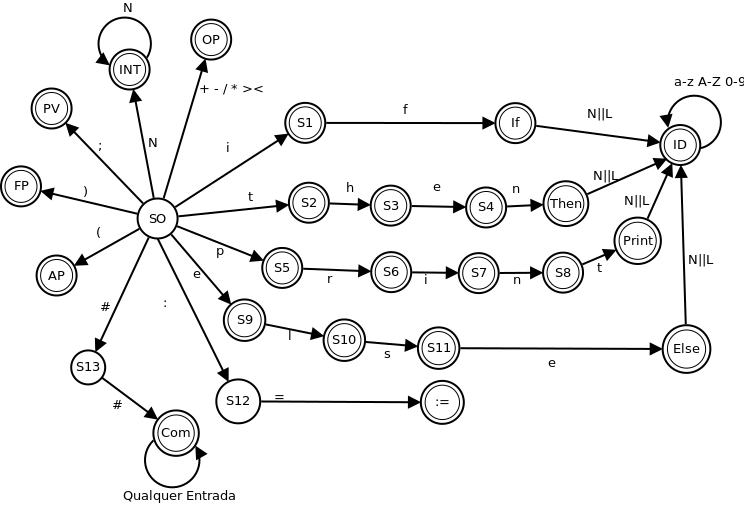
\includegraphics[scale=0.55]{AutomatoLexico.png}
\end{center}


\\Automato - Ocaml
\begin{lstlisting}
let lexico (str:entrada) = 
  let trans (e:estado) (c:simbolo) = 
match (e,c) with    
    | (0, 'i') -> 1
    | (0, 't') -> 6
    | (0, 'e') -> 10
    | (0, 'p') -> 14
    | (0, 'f') -> 25
    | (0, 'w') -> 28
    | (0, '(') -> 19
    | (0, ')') -> 20
    | (0, ';') -> 22
    | (0, ':') -> 23
    | (0, '#') -> 33
    | (0, _) when eh_operador c -> 21
    | (0, _) when eh_letra c -> 3
    | (0, _) when eh_digito c -> 4
    | (0, _) when eh_branco c -> 5 
    | (0, _) -> failwith ("Erro lexico: caracter desconhecido " ^ Char.escaped c)
    
    | (1, 'f') -> 2
    | (1, _) when eh_letra c || eh_digito c -> 3
    
    | (2, _) when eh_letra c || eh_digito c -> 3
    
    | (3, _) when eh_letra c || eh_digito c -> 3
    
    | (4, _) when eh_digito c -> 4
    
    | (5, _) when eh_branco c -> 5
    
    | (6, 'h') -> 7
    | (6, _) when eh_letra c || eh_digito c -> 3
   
    | (7, 'e') -> 8
    | (7, _)  when eh_letra c || eh_digito c -> 3
    
    | (8, 'n') -> 9  
    | (8, _)  when eh_letra c || eh_digito c -> 3

    | (9, _)  when eh_letra c || eh_digito c -> 3

    | (10, 'l') -> 11
    | (10, _) when eh_letra c || eh_digito c -> 3
    
    | (11, 's') -> 12
    | (11, _)  when eh_letra c || eh_digito c -> 3
    
    | (12, 'e') -> 13 
    | (12, _)  when eh_letra c || eh_digito c -> 3
    
    | (13, _)  when eh_letra c || eh_digito c -> 3

    | (14, 'r') -> 15
    | (14, _) when eh_letra c || eh_digito c -> 3
    
    | (15, 'i') -> 16
    | (15, _)  when eh_letra c || eh_digito c -> 3
    
    | (16, 'n') -> 17 
    | (16, _)  when eh_letra c || eh_digito c -> 3
    
    | (17, 't') -> 18
    | (17, _)  when eh_letra c || eh_digito c -> 3
    
    | (18, _)  when eh_letra c || eh_digito c -> 3

    | (23,'=') -> 24

    | (25, 'o') -> 26
    | (25, _)  when eh_letra c || eh_digito c -> 3

    | (26, 'r') -> 27
    | (27, _)  when eh_letra c || eh_digito c -> 3

    | (27, _)  when eh_letra c || eh_digito c -> 3

    | (28, 'h') -> 29
    | (28, _)  when eh_letra c || eh_digito c -> 3
    
    | (29, 'i') -> 30
    | (29, _)  when eh_letra c || eh_digito c -> 3

    | (30, 'l') -> 31
    | (30, _)  when eh_letra c || eh_digito c -> 3
    
    | (31, 'e') -> 32
    | (31, _)  when eh_letra c || eh_digito c -> 3

    | (32, _)  when eh_letra c || eh_digito c -> 3

    | (33, '#') -> 34

    | (34, _) when pulou_linha c -> 0
    | (34, _) -> 34


    | _ -> estado_morto
 and rotulo e str =
  match e with
  | 2 -> If
  | 1 
  | 6
  | 7
  | 8
  | 10
  | 11
  | 12
  | 14
  | 15
  | 16
  | 17
  | 25
  | 26
  | 28
  | 29
  | 30
  | 31
  | 3 -> Id str
  | 4 -> Int str
  | 5 -> Branco
  | 9 -> Then
  | 13 -> Else
  | 18 -> Print
  | 19 -> APar
  | 20 -> FPar
  | 21 -> OP str
  | 22 -> PV
  | 24 -> Atrib
  | 27 -> For
  | 32 -> While
  | _ -> failwith ("Erro lexico: sequencia desconhecida " ^ str)
in let dfa = { transicao = trans;
               estado = estado_inicial;
               posicao = 0 }
in let estado_lexico = {
  pos_inicial = 0;
  pos_final = -1;
  ultimo_final = -1;
  rotulo = rotulo;
  dfa = dfa
} in
  analisador str (String.length str) estado_lexico
\end{lstlisting}
Seguem as funções principais feitas pelo professor que viabilizaram o fun-
cionamento da função léxico:

\begin{itemize}
\item obtem\_token\_e\_estado: função responsável por atualizar o autômato
para o próximo estado dado uma string e um estado léxico como parâmetro.
\item analisador: responsável por analisar o estado corrente do estado léxico.
Se estivermos no estado final, paramos, caso contrario, se estivermos
no estado morto, vamos para o proximo estado e verificamos qual ele
é 
\end{itemize}

Analisador Lexico
\subsubsection{Implementação}
Este analisador foi implementado utilizando a linguagem funcional Ocaml. Segue no código abaixo, todas as funções utilizadas para a implementação do mesmo para que possam ser reconhecidas as empressões encontradas na sessão 
\hyperref[sec:abordagem]{7.1}
\begin{lstlisting}
{

  open Lexing
  open Printf

  type token =
  | LITINT of (int)
  | LITSTRING of (string)
  | ID of (string)
  | LITFLOAT of (float)
  | APAR
  | FPAR
  | VIRG
  | MAIS
  | DPONTOS
  | MENORIGUAL
  | SETA
  | E
  | ATRIB
  | RETURN
  | DEF
  | EOF
  (*tokens adicionados*)
  | OU
  | IF
  | ELSE
  | WHILE
  | FOR
  | MAIORIGUAL
  | IMPORT
  | INT
  | FLOAT
  | LIST
  | ABRECOLCHETES
  | FECHACOLCHETES
  | ABRECHAVES
  | FECHACHAVES
  | INCR 
  | DECR 
  | IGUALDADE
  | MENOS
  | VEZES
  | DIVIDIDO
  | MENOR
  | MAIOR
  | PV
  | IN
  | RANGE
  | CHAR
  | DOUBLE
  | PONTO
  | PASS
  | VOID
  | ELIF
  | PRINT
  | STR
  | INPUT
  | LENGTH
  | DIFERENTE
  | TRUE
  | FALSE
  | BREAK
  | IS
  | NOT
  | MODULO
  | FROM
  | ATRIBMAIS 
  | ATRIBMENOS 
  | ATRIBMULT 
  | ATRIBDIV 
  (* Os tokens a seguir são importantes para o pré processador *)
  | Linha of (int * int * token list)
  | INDENTA
  | DEDENTA
  | NOVALINHA

  (*Adicionado*)
  let booleano nbool = 
    match nbool with
      | "True" -> 1
      | "False" -> 0
      | _ -> failwith "Erro: nao eh valor booleano"  

  let nivel_par = ref 0

  let incr_num_linha lexbuf =
    let pos = lexbuf.lex_curr_p in
      lexbuf.lex_curr_p <- { pos with
         pos_lnum = pos.pos_lnum + 1;
         pos_bol = pos.pos_cnum;
      }

  let msg_erro lexbuf c =
    let pos = lexbuf.lex_curr_p in
    let lin = pos.pos_lnum
    and col = pos.pos_cnum - pos.pos_bol - 1 in
    sprintf "%d-%d: caracter desconhecido %c" lin col c

  (*Adicionado*)
  let erro lin col msg =
    let mensagem = sprintf "%d-%d: %s" lin col msg in
       failwith mensagem


}

let digito = ['0' - '9']
let int =  digito+
let comentario = "#"[ ^ '\n' ]*
let linha_em_branco = [' ' '\t' ]* comentario
let restante = [^ ' ' '\t' '\n' ] [^ '\n']+
let brancos = [' ' '\t']+
let novalinha = '\r' | '\n' | "\r\n"
let letra = [ 'a'-'z' 'A' - 'Z']
let identificador = letra ( letra | digito | '_' )*

(* O pré processador necessário para contabilizar a identação *)
rule preprocessador indentacao = parse
  linha_em_branco         { preprocessador 0 lexbuf } (* ignora brancos *)
| [' ' '\t' ]+ '\n'       { incr_num_linha lexbuf;
                            preprocessador 0 lexbuf } (* ignora brancos *)
| ' '                     { preprocessador (indentacao + 1) lexbuf }
| '\t'                    { let nova_ind = indentacao + 8 - (indentacao mod 8) 
                            in preprocessador nova_ind lexbuf }
| novalinha               { incr_num_linha lexbuf;
                            preprocessador 0 lexbuf }
| restante as linha {
      let rec tokenize lexbuf =
          let tok = token lexbuf in
	  match tok with
	     EOF -> []
	 | _ -> tok :: tokenize lexbuf in
      let toks = tokenize (Lexing.from_string linha) in
      (* A impressão a seguir serve apenas para depuração. Retirar depois! *)
      printf "Linha(identacao=%d,nivel_par=%d)\n" indentacao (!nivel_par);
      Linha(indentacao,!nivel_par, toks)
}
| eof { nivel_par := 0; EOF }




(* O analisador léxico a ser chamado após o pré processador *)
and token = parse
  brancos            { token lexbuf }
| comentario         { token lexbuf }
| "'''"               { comentario_bloco 0 lexbuf; }
| ">="               { MAIORIGUAL}
| "<="               { MENORIGUAL }
| "->"               { SETA }
| "++"               { INCR }
| "--"               { DECR }
| "=="               { IGUALDADE }
| "!="               { DIFERENTE }
| "+="               { ATRIBMAIS }
| "-="               { ATRIBMENOS }
| "*="               { ATRIBMULT }
| "/="               { ATRIBDIV }
| '{'                { ABRECHAVES }
| '}'                { FECHACHAVES }
| '['                { ABRECOLCHETES }
| ']'                { FECHACOLCHETES }
| '('                { let _ = incr(nivel_par) in APAR }
| ')'                { let _ = decr(nivel_par) in FPAR }
| ','                { VIRG }
| '+'                { MAIS  }
| '-'                { MENOS  }
| '*'                { VEZES  }
| '/'                { DIVIDIDO }
| '='                { ATRIB }
| ':'                { DPONTOS }
| ';'                { PV }
| '<'                { MENOR }
| '>'                { MAIOR }
| '%'		             { MODULO }
| '.'                { PONTO }
| int as num         { let numero = int_of_string num in
                       LITINT numero }                    
| "or"               { OU }
| "if"               { IF }
| "else"             { ELSE }
| "while"            { WHILE }
| "for"              { FOR }
| "return"           { RETURN }
| "def"              { DEF }
| "import"           { IMPORT }
| "int"              { INT }
| "float"            { FLOAT }
| "double"           { DOUBLE }
| "char"             { CHAR }
| "list"             { LIST }
| "and"              { E    }
| "in"               { IN }
| "range"            { RANGE }
| "pass"             { PASS }
| "void"             { VOID }
| "elif"	           { ELIF }
| "print"            { PRINT }
| "str"              { STR }
| "input"            { INPUT }
| "len"              { LENGTH }
| "break"            { BREAK }
| "is"               { IS }
| "not"		           { NOT }
| "from"	           { FROM }
| identificador as id { ID id }
| '"'                { let pos = lexbuf.lex_curr_p in
                       let lin = pos.pos_lnum
                       and col = pos.pos_cnum - pos.pos_bol - 1 in
                       let buffer = Buffer.create 1 in 
                       let str = leia_string lin col buffer lexbuf in
                           LITSTRING str }
| _ as c  { failwith (msg_erro lexbuf c) }
| eof        { EOF }



and comentario_bloco n = parse
   "'''"      { if n=0 then token lexbuf 
               else comentario_bloco (n-1) lexbuf }
| "'''"       { comentario_bloco (n+1) lexbuf }
| novalinha  { incr_num_linha lexbuf; comentario_bloco n lexbuf }
| _          { comentario_bloco n lexbuf }
| eof        { failwith "Comentário não fechado" }



and leia_string lin col buffer = parse
    | '"'     { Buffer.contents buffer}
    | "\\t"    { Buffer.add_char buffer '\t'; leia_string lin col buffer lexbuf }
    | "\\n"    { Buffer.add_char buffer '\n'; leia_string lin col buffer lexbuf }
    | '\\' '"'  { Buffer.add_char buffer '"'; leia_string lin col buffer lexbuf }
    | '\\' '\\' { Buffer.add_char buffer '\\'; leia_string lin col buffer lexbuf }
    | _ as c    { Buffer.add_char buffer c; leia_string lin col buffer lexbuf }
    | eof      { erro lin col "A string não foi fechada"}




\end{lstlisting}



\subsubsection{Execução}
Para que possa executar o analisador léxico, deve estar instalado o Ocaml. Seu tutorial
de instalação encontra-se em 4.2\\\\

1. Deve-se no terminal, compilar o arquivo lexico.mll para gerar o arquivo lexico.ml, utilizando o comando::\\
\fbox{\textbf{ocamllex lexico.mll}}\\\\

2. Agora, o compilador do OCaml deve compilar o arquivo lexico.ml, gerando o arquivo
"carregador.ml", utilizando o comando:\\
\fbox{\textbf{ocamlc -c lexico.ml}}\\\\

3. Já compilado, deve-se abrir o OCaml utilizando o seguinte comando:\\
\fbox{\textbf{ocaml}}\\\\

4. Para que o OCaml possa carregar o analisador léxico, utilizando o seguinte co-
mando:\\
\fbox{\textbf{\#use "carregador.ml";;}}\\\\

5. Neste momento já é possível testá-lo. Pode-se utilizar da seguinte forma, para analisar
o codigo escrito em um arquivo chamado "codigo":\\
\fbox{\textbf{lex "codigo";}}\\\\


Supondo o seguinte arquivo de código abaixo:

\begin{lstlisting}
def paco(x):
    x = x + 1
    y = x + 2
    y = x + 3 + ( 4
 + 5)
  return x
\end{lstlisting}

\\\\A saída do analisador léxico é a seguinte:
\begin{lstlisting}
Linha(identacao=0,nivel_par=0)
Nivel: 0
Linha(identacao=8,nivel_par=0)
Nivel: 8
Linha(identacao=8,nivel_par=0)
Nivel: 8
Linha(identacao=8,nivel_par=0)
Nivel: 8
Linha(identacao=8,nivel_par=0)
Nivel: 8
EOF
- : tokens =
            [Lexico.DEF; Lexico.ID "paco"; Lexico.APAR; 
            Lexico.ID "x"; Lexico.FPAR;Lexico.DPONTOS; 
            Lexico.NOVALINHA; Lexico.INDENTA; Lexico.ID "x";
            Lexico.ATRIB; Lexico.ID "x"; Lexico.MAIS; 
            Lexico.LITINT 1; Lexico.NOVALINHA;Lexico.ID "y";
            Lexico.ATRIB; Lexico.ID "x"; Lexico.MAIS; 
            Lexico.LITINT 2;Lexico.NOVALINHA; Lexico.ID "y";
            Lexico.ATRIB; Lexico.ID "x"; Lexico.MAIS;
            Lexico.LITINT 3; Lexico.MAIS; Lexico.APAR;
            Lexico.LITINT 4; Lexico.MAIS;Lexico.LITINT 5;
            Lexico.FPAR; Lexico.NOVALINHA; Lexico.RETURN;
            Lexico.ID "x"; Lexico.NOVALINHA; Lexico.DEDENTA;
            Lexico.EOF]
\end{lstlisting}

\subsection{Abordagem por Linguagem Regular}
Foi feita uma implementação de linguagem regula.Dessa forma facilita
o processo de análise léxica.\\\\

\subsubsection{Implementação}
Os principais tokens são NOVALINHA, IDENTA e DEDENTA que re-
alizam o controle de identação do python. NOVALINHA é inserido após
a quebra de linha e pode ser seguido do identa caso algum comando seja
dado. EX.: for, while, ou seja, comandos que exigem identação, O token
DEDENTA é utilizado toda a vez a identação volta ao normal o que significa
o fim de um comando.\\\\
Fazendo uma analogia com a linguagem C, pode-se dizer que o token
NOVALINHA representa a vı́rgula, IDENTA representa abrir chaves e DE-
DENTA, fechar chaves.
%%%%%%%%%%%%%%%%%%%%%%%%%%%%%%%%%%%%%%%%%%%%%%%%%%%%%%%%%%%%%%%%%%%%%%%%%%
\subsubsection{Execução}
\\\\\\Código    
\begin{lstlisting}
def nano02():
	n = int n)
\end{lstlisting}

\\Saída
\begin{lstlisting}
# lex "nano02.py";;
Linha(identacao=0,nivel_par=0)
Nivel: 0
Linha(identacao=8,nivel_par=-1)
Nivel: 8
EOF
- : tokens =
[Lexico.DEF; Lexico.ID "nano02"; Lexico.APAR; Lexico.FPAR; Lexico.DPONTOS;
 Lexico.NOVALINHA; Lexico.INDENTA; Lexico.ID "n"; Lexico.ATRIB; Lexico.INT;
 Lexico.ID "n"; Lexico.FPAR; Lexico.DEDENTA; Lexico.EOF]
\end{lstlisting}
%%%%%%%%%%%%%%%%%%%%%%%%%%%%%%%%%%%%%%%%%%%%%%%%%%%%%%%%%%%%%%%%%%%%%%%%%%
\\\\\\Código
\begin{lstlisting}
def nano03():
	n = int(n)
	n=1
\end{lstlisting}

\\Saída
\begin{lstlisting}
Linha(identacao=0,nivel_par=0)
Nivel: 0
Linha(identacao=8,nivel_par=0)
Nivel: 8
Linha(identacao=8,nivel_par=0)
Nivel: 8
EOF
- : tokens =
[Lexico.DEF; Lexico.ID "nano03"; Lexico.APAR; Lexico.FPAR; Lexico.DPONTOS;
 Lexico.NOVALINHA; Lexico.INDENTA; Lexico.ID "n"; Lexico.ATRIB; Lexico.INT;
 Lexico.APAR; Lexico.ID "n"; Lexico.FPAR; Lexico.NOVALINHA; Lexico.ID "n";
 Lexico.ATRIB; Lexico.LITINT 1; Lexico.NOVALINHA; Lexico.DEDENTA; Lexico.EOF]
\end{lstlisting}
%%%%%%%%%%%%%%%%%%%%%%%%%%%%%%%%%%%%%%%%%%%%%%%%%%%%%%%%%%%%%%%%%%%%%%%%%%
\\
\\
Código
\begin{lstlisting}
def nano03():
	n = int(n)
	n=1
\end{lstlisting}

\\Saída
\begin{lstlisting}
Linha(identacao=0,nivel_par=0)
Nivel: 0
Linha(identacao=8,nivel_par=0)
Nivel: 8
Linha(identacao=8,nivel_par=0)
Nivel: 8
EOF
- : tokens =
[Lexico.DEF; Lexico.ID "nano03"; Lexico.APAR; Lexico.FPAR; Lexico.DPONTOS;
 Lexico.NOVALINHA; Lexico.INDENTA; Lexico.ID "n"; Lexico.ATRIB; Lexico.INT;
 Lexico.APAR; Lexico.ID "n"; Lexico.FPAR; Lexico.NOVALINHA; Lexico.ID "n";
 Lexico.ATRIB; Lexico.LITINT 1; Lexico.NOVALINHA; Lexico.DEDENTA; Lexico.EOF]
\end{lstlisting}
%%%%%%%%%%%%%%%%%%%%%%%%%%%%%%%%%%%%%%%%%%%%%%%%%%%%%%%%%%%%%%%%%%%%%%%%%%
\\\\\\Código
\begin{lstlisting}
def nano04():
	n = int(n)
	n = 1 + 2 
\end{lstlisting}

\\Saída
\begin{lstlisting}
Linha(identacao=0,nivel_par=0)
Nivel: 0
Linha(identacao=8,nivel_par=0)
Nivel: 8
Linha(identacao=8,nivel_par=0)
Nivel: 8
EOF
- : tokens =
[Lexico.DEF; Lexico.ID "nano04"; Lexico.APAR; Lexico.FPAR; Lexico.DPONTOS;
 Lexico.NOVALINHA; Lexico.INDENTA; Lexico.ID "n"; Lexico.ATRIB; Lexico.INT;
 Lexico.APAR; Lexico.ID "n"; Lexico.FPAR; Lexico.NOVALINHA; Lexico.ID "n";
 Lexico.ATRIB; Lexico.LITINT 1; Lexico.MAIS; Lexico.LITINT 2;
 Lexico.NOVALINHA; Lexico.DEDENTA; Lexico.EOF]
\end{lstlisting}
%%%%%%%%%%%%%%%%%%%%%%%%%%%%%%%%%%%%%%%%%%%%%%%%%%%%%%%%%%%%%%%%%%%%%%%%%%
\\\\\\Código
\begin{lstlisting}
def nano05():
	n = 2 
	print(n,end="")
	
nano05()
\end{lstlisting}

\\Saída
\begin{lstlisting}
Linha(identacao=0,nivel_par=0)
Nivel: 0
Linha(identacao=8,nivel_par=0)
Nivel: 8
Linha(identacao=8,nivel_par=0)
Nivel: 8
Linha(identacao=0,nivel_par=0)
Nivel: 0
EOF
- : tokens =
[Lexico.DEF; Lexico.ID "nano05"; Lexico.APAR; Lexico.FPAR; Lexico.DPONTOS;
 Lexico.NOVALINHA; Lexico.INDENTA; Lexico.ID "n"; Lexico.ATRIB;
 Lexico.LITINT 2; Lexico.NOVALINHA; Lexico.PRINT; Lexico.APAR; Lexico.ID "n";
 Lexico.VIRG; Lexico.ID "end"; Lexico.ATRIB; Lexico.LITSTRING "";
 Lexico.FPAR; Lexico.NOVALINHA; Lexico.DEDENTA; Lexico.ID "nano05";
 Lexico.APAR; Lexico.FPAR; Lexico.NOVALINHA; Lexico.EOF]
\end{lstlisting}
%%%%%%%%%%%%%%%%%%%%%%%%%%%%%%%%%%%%%%%%%%%%%%%%%%%%%%%%%%%%%%%%%%%%%%%%%%

\\\\\\Código
\begin{lstlisting}
def nano06():
	n = 1 - 2 
	print(n,end="")

nano06()
\end{lstlisting}

\\Saída
\begin{lstlisting}
Linha(identacao=0,nivel_par=0)
Nivel: 0
Linha(identacao=8,nivel_par=0)
Nivel: 8
Linha(identacao=8,nivel_par=0)
Nivel: 8
Linha(identacao=0,nivel_par=0)
Nivel: 0
EOF
- : tokens =
[Lexico.DEF; Lexico.ID "nano06"; Lexico.APAR; Lexico.FPAR; Lexico.DPONTOS;
 Lexico.NOVALINHA; Lexico.INDENTA; Lexico.ID "n"; Lexico.ATRIB;
 Lexico.LITINT 1; Lexico.MENOS; Lexico.LITINT 2; Lexico.NOVALINHA;
 Lexico.PRINT; Lexico.APAR; Lexico.ID "n"; Lexico.VIRG; Lexico.ID "end";
 Lexico.ATRIB; Lexico.LITSTRING ""; Lexico.FPAR; Lexico.NOVALINHA;
 Lexico.DEDENTA; Lexico.ID "nano06"; Lexico.APAR; Lexico.FPAR;
 Lexico.NOVALINHA; Lexico.EOF]
\end{lstlisting}

%%%%%%%%%%%%%%%%%%%%%%%%%%%%%%%%%%%%%%%%%%%%%%%%%%%%%%%%%%%%%%%%%%%%%%%%%%

\\\\\\Código
\begin{lstlisting}
def nano07():
	n=1
	if n ==1:
		print(n,end="")

nano07()
\end{lstlisting}

\\Saída
\begin{lstlisting}
Linha(identacao=0,nivel_par=0)
Nivel: 0
Linha(identacao=8,nivel_par=0)
Nivel: 8
Linha(identacao=8,nivel_par=0)
Nivel: 8
Linha(identacao=16,nivel_par=0)
Nivel: 16
Linha(identacao=0,nivel_par=0)
Nivel: 0
EOF
- : tokens =
[Lexico.DEF; Lexico.ID "nano07"; Lexico.APAR; Lexico.FPAR; Lexico.DPONTOS;
 Lexico.NOVALINHA; Lexico.INDENTA; Lexico.ID "n"; Lexico.ATRIB;
 Lexico.LITINT 1; Lexico.NOVALINHA; Lexico.IF; Lexico.ID "n";
 Lexico.IGUALDADE; Lexico.LITINT 1; Lexico.DPONTOS; Lexico.NOVALINHA;
 Lexico.INDENTA; Lexico.PRINT; Lexico.APAR; Lexico.ID "n"; Lexico.VIRG;
 Lexico.ID "end"; Lexico.ATRIB; Lexico.LITSTRING ""; Lexico.FPAR;
 Lexico.NOVALINHA; Lexico.DEDENTA; Lexico.DEDENTA; Lexico.ID "nano07";
 Lexico.APAR; Lexico.FPAR; Lexico.NOVALINHA; Lexico.EOF]
\end{lstlisting}


%%%%%%%%%%%%%%%%%%%%%%%%%%%%%%%%%%%%%%%%%%%%%%%%%%%%%%%%%%%%%%%%%%%%%%%%%%

\\\\\\Código
\begin{lstlisting}
def nano08():
	n=1
	if n ==1:
		print(n,end="")
	else:
		print(0,end="")

nano08()
\end{lstlisting}

\\Saída
\begin{lstlisting}
Linha(identacao=0,nivel_par=0)
Nivel: 0
Linha(identacao=8,nivel_par=0)
Nivel: 8
Linha(identacao=8,nivel_par=0)
Nivel: 8
Linha(identacao=16,nivel_par=0)
Nivel: 16
Linha(identacao=8,nivel_par=0)
Nivel: 8
Linha(identacao=16,nivel_par=0)
Nivel: 16
Linha(identacao=0,nivel_par=0)
Nivel: 0
EOF
- : tokens =
[Lexico.DEF; Lexico.ID "nano08"; Lexico.APAR; Lexico.FPAR; Lexico.DPONTOS;
 Lexico.NOVALINHA; Lexico.INDENTA; Lexico.ID "n"; Lexico.ATRIB;
 Lexico.LITINT 1; Lexico.NOVALINHA; Lexico.IF; Lexico.ID "n";
 Lexico.IGUALDADE; Lexico.LITINT 1; Lexico.DPONTOS; Lexico.NOVALINHA;
 Lexico.INDENTA; Lexico.PRINT; Lexico.APAR; Lexico.ID "n"; Lexico.VIRG;
 Lexico.ID "end"; Lexico.ATRIB; Lexico.LITSTRING ""; Lexico.FPAR;
 Lexico.NOVALINHA; Lexico.DEDENTA; Lexico.ELSE; Lexico.DPONTOS;
 Lexico.NOVALINHA; Lexico.INDENTA; Lexico.PRINT; Lexico.APAR;
 Lexico.LITINT 0; Lexico.VIRG; Lexico.ID "end"; Lexico.ATRIB;
 Lexico.LITSTRING ""; Lexico.FPAR; Lexico.NOVALINHA; Lexico.DEDENTA;
 Lexico.DEDENTA; Lexico.ID "nano08"; Lexico.APAR; Lexico.FPAR;
 Lexico.NOVALINHA; Lexico.EOF]
\end{lstlisting}


%%%%%%%%%%%%%%%%%%%%%%%%%%%%%%%%%%%%%%%%%%%%%%%%%%%%%%%%%%%%%%%%%%%%%%%%%%

\\\\\\Código
\begin{lstlisting}
def nano09():
	n=1
	if n ==1:
		print(n,end="")
	else:
		print(0,end="")

nano09()
\end{lstlisting}

\\Saída
\begin{lstlisting}
Linha(identacao=0,nivel_par=0)
Nivel: 0
Linha(identacao=8,nivel_par=0)
Nivel: 8
Linha(identacao=8,nivel_par=0)
Nivel: 8
Linha(identacao=16,nivel_par=0)
Nivel: 16
Linha(identacao=8,nivel_par=0)
Nivel: 8
Linha(identacao=16,nivel_par=0)
Nivel: 16
Linha(identacao=0,nivel_par=0)
Nivel: 0
EOF
- : tokens =
[Lexico.DEF; Lexico.ID "nano09"; Lexico.APAR; Lexico.FPAR; Lexico.DPONTOS;
 Lexico.NOVALINHA; Lexico.INDENTA; Lexico.ID "n"; Lexico.ATRIB;
 Lexico.LITINT 1; Lexico.NOVALINHA; Lexico.IF; Lexico.ID "n";
 Lexico.IGUALDADE; Lexico.LITINT 1; Lexico.DPONTOS; Lexico.NOVALINHA;
 Lexico.INDENTA; Lexico.PRINT; Lexico.APAR; Lexico.ID "n"; Lexico.VIRG;
 Lexico.ID "end"; Lexico.ATRIB; Lexico.LITSTRING ""; Lexico.FPAR;
 Lexico.NOVALINHA; Lexico.DEDENTA; Lexico.ELSE; Lexico.DPONTOS;
 Lexico.NOVALINHA; Lexico.INDENTA; Lexico.PRINT; Lexico.APAR;
 Lexico.LITINT 0; Lexico.VIRG; Lexico.ID "end"; Lexico.ATRIB;
 Lexico.LITSTRING ""; Lexico.FPAR; Lexico.NOVALINHA; Lexico.DEDENTA;
 Lexico.DEDENTA; Lexico.ID "nano09"; Lexico.APAR; Lexico.FPAR;
 Lexico.NOVALINHA; Lexico.EOF]
\end{lstlisting}


%%%%%%%%%%%%%%%%%%%%%%%%%%%%%%%%%%%%%%%%%%%%%%%%%%%%%%%%%%%%%%%%%%%%%%%%%%
\\\\\\Código
\begin{lstlisting}
def nano10():
	n=1 
	m=2
	if n ==m:
		print(n,end="")
	else:
		print(0,end="")


nano10()
\end{lstlisting}

\\Saída
\begin{lstlisting}
Linha(identacao=0,nivel_par=0)
Nivel: 0
Linha(identacao=8,nivel_par=0)
Nivel: 8
Linha(identacao=8,nivel_par=0)
Nivel: 8
Linha(identacao=8,nivel_par=0)
Nivel: 8
Linha(identacao=16,nivel_par=0)
Nivel: 16
Linha(identacao=8,nivel_par=0)
Nivel: 8
Linha(identacao=16,nivel_par=0)
Nivel: 16
Linha(identacao=0,nivel_par=0)
Nivel: 0
EOF
- : tokens =
[Lexico.DEF; Lexico.ID "nano10"; Lexico.APAR; Lexico.FPAR; Lexico.DPONTOS;
 Lexico.NOVALINHA; Lexico.INDENTA; Lexico.ID "n"; Lexico.ATRIB;
 Lexico.LITINT 1; Lexico.NOVALINHA; Lexico.ID "m"; Lexico.ATRIB;
 Lexico.LITINT 2; Lexico.NOVALINHA; Lexico.IF; Lexico.ID "n";
 Lexico.IGUALDADE; Lexico.ID "m"; Lexico.DPONTOS; Lexico.NOVALINHA;
 Lexico.INDENTA; Lexico.PRINT; Lexico.APAR; Lexico.ID "n"; Lexico.VIRG;
 Lexico.ID "end"; Lexico.ATRIB; Lexico.LITSTRING ""; Lexico.FPAR;
 Lexico.NOVALINHA; Lexico.DEDENTA; Lexico.ELSE; Lexico.DPONTOS;
 Lexico.NOVALINHA; Lexico.INDENTA; Lexico.PRINT; Lexico.APAR;
 Lexico.LITINT 0; Lexico.VIRG; Lexico.ID "end"; Lexico.ATRIB;
 Lexico.LITSTRING ""; Lexico.FPAR; Lexico.NOVALINHA; Lexico.DEDENTA;
 Lexico.DEDENTA; Lexico.ID "nano10"; Lexico.APAR; Lexico.FPAR;
 Lexico.NOVALINHA; Lexico.EOF]

\end{lstlisting}
%%%%%%%%%%%%%%%%%%%%%%%%%%%%%%%%%%%%%%%%%%%%%%%%%%%%%%%%%%%%%%%%%%%%%%%%%%

\subsubsection{Erros Léxicos}
\\\\\\Código
\begin{lstlisting}
def micro01():
	cel , far = 0.0 , 0.0
	print("		Tabela de conversao: Celsius -> Fahrenheit")
	print("Digite a temperatura em Celsius: ",end="")
	cel = input()
	far = (9*cel+160)/5
	print("A nova temperatura eh:"+str(far)+"F)
	''' cine'''
micro01()
\end{lstlisting}

\\Saída
\\Erro: String Aberta
\begin{lstlisting}
Linha(identacao=0,nivel_par=0)
Nivel: 0
Linha(identacao=8,nivel_par=0)
Nivel: 8
Linha(identacao=8,nivel_par=0)
Nivel: 8
Linha(identacao=8,nivel_par=0)
Nivel: 8
Linha(identacao=8,nivel_par=0)
Nivel: 8
Linha(identacao=8,nivel_par=0)
Nivel: 8

Exception: Failure "1-40: A string nao foi fechada".
\end{lstlisting}
%%%%%%%%%%%%%%%%%%%%%%%%%%%%%%%%%%%%%%%%%%%%%%%%%%%%%%%%%%%%%%%%%%%%%%%%%%

\\\\\\Código
\begin{lstlisting}
def micro01():
	@cel , far = 0.0 , 0.0
	print("		Tabela de conversao: Celsius -> Fahrenheit")
	print("Digite a temperatura em Celsius: ",end="")
	cel = input()
	far = (9*cel+160)/5
	print("A nova temperatura eh:"+str(far)+"F")
	''' cine'''
micro01()
\end{lstlisting}

\\Saída
\\Erro: Variável com caractere proibido
\begin{lstlisting}
Linha(identacao=0,nivel_par=0)
Nivel: 0

Exception: Failure "1-0: caracter desconhecido @".
\end{lstlisting}
%%%%%%%%%%%%%%%%%%%%%%%%%%%%%%%%%%%%%%%%%%%%%%%%%%%%%%%%%%%%%%%%%%%%%%%%%%

\\\\\\Código
\begin{lstlisting}
def micro01():
	cel , far = 0.0 , 0.0
	print("		Tabela de conversao: Celsius -> Fahrenheit")
	print("Digite a temperatura em Celsius: ",end="")
	cel = input()
	far = (9*cel+160)/5
	print("A nova temperatura eh:"+str(far)+"F")
	''' cine
	
micro01()
\end{lstlisting}

\\Saída
\\Erro: Comentario não fechado
\begin{lstlisting}
Linha(identacao=0,nivel_par=0)
Nivel: 0
Linha(identacao=8,nivel_par=0)
Nivel: 8
Linha(identacao=8,nivel_par=0)
Nivel: 8
Linha(identacao=8,nivel_par=0)
Nivel: 8
Linha(identacao=8,nivel_par=0)
Nivel: 8
Linha(identacao=8,nivel_par=0)
Nivel: 8
Linha(identacao=8,nivel_par=0)
Nivel: 8

Exception: Failure "Comentario nao fechado".
\end{lstlisting}
%%%%%%%%%%%%%%%%%%%%%%%%%%%%%%%%%%%%%%%%%%%%%%%%%%%%%%%%%%%%%%%%%%%%%%%%%%



\section{Analisador Sintático}
Essa seção contém a implementação de um analisador sintático simples abordado em sala de aula e ourto para mini-Python.\\\

\subsection{Analisador Abordado em Aula}

\subsubsection{Gramática}
Como passo inicial foi passado em sala de aula, pelo professor Alexssandro Santos Soares, a gramática a seguir com o intuito de aprofundarmos os conhecimentos do processo da análise.\\\

{\raggedright
S -> XYZ\\
X -> aXb\\
X ->\\
Y -> cYZcX\\
Y -> d\\
Z -> eZYe\\
Z -> f\\
}
\\
\
\\Para que seja melhor o entendimento da proxima tabela precisamos entender os conceitos de first e follow.
First: conjunto de sı́mbolos que ocorrem no inı́cio de uma determinada regra.\\ 
Follow: o que pode aparecer depois da ocorrência de um determinado sı́mbolo.\\

\begin{center}
    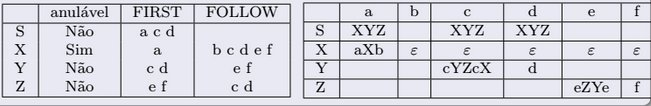
\includegraphics[scale=0.5]{TabelaSintatico.jpg}
    figura 1
\end{center}

\subsubsection{Código}
Segue os códigos do analisador sintático, juntamente com os arquivos lexico.mll (o qual usaremos para efetuar analise do capitulo anterior) e sintatico.mli(tokens para efetuar a analise sintativa) e o sintativoArv.ml(contrução da arvore sintátiva para efetuarmos a analise).\\

\\\\\\léxico.mll
\begin{lstlisting}
{
  open Lexing
  open Printf
  open Sintatico
         
  let incr_num_linha lexbuf = 
    let pos = lexbuf.lex_curr_p in
     lexbuf.lex_curr_p <- { pos with
        pos_lnum = pos.pos_lnum + 1;
        pos_bol = pos.pos_cnum;
     }

  let msg_erro lexbuf c =
    let pos = lexbuf.lex_curr_p in
    let lin = pos.pos_lnum
    and col = pos.pos_cnum - pos.pos_bol - 1 in
    sprintf "%d-%d: caracter desconhecido %c" lin col c

}

rule token = parse 
| 'a'        {A}
| 'b'        {B}
| 'c'        {C}
| 'd'        {D}
| 'e'        {E}
| 'f'        {F}
| _ as c  { failwith (msg_erro lexbuf c) }
| eof        { EOF }
\end{lstlisting}


\\\\\\sintaticoArv.ml
\begin{lstlisting}
(* Parser preditivo *)
#load "lexico.cmo";;
open Sintatico;;

type rule = S of rule * rule * rule
            | X of tokens * rule * tokens
            | Y of tokens * rule * rule * tokens * rule
            | Z of tokens * rule * rule * tokens
            | X_vazio
            | Y_d of tokens
            | Z_f of tokens

let tk = ref EOF (* variavel global para o token atual *)
let lexbuf = ref (Lexing.from_string "")

(* le o proximo token *)             
let prox () = tk := Lexico.token !lexbuf
                                 
let to_str tk =
  match tk with
    A -> "a"
  | B -> "b"
  | C -> "c"
  | D -> "d"
  | E -> "e"
  | F -> "f"
  | EOF -> "eof"

let erro esp =
  let msg = Printf.sprintf "Erro: esperava %s mas encontrei %s"
                            esp (to_str !tk)
  in
  failwith msg

let consome t = if (!tk == t) then prox() else erro (to_str t)
                                                   
let rec ntS () =
  match !tk with
    A    
   |C     
   |D     -> 
             let cmd1 = ntX() in
             let cmd2 = ntY() in
             let cmd3 = ntZ() in
             S (cmd1, cmd2, cmd3)
  | _ -> erro "a, c ou d"
and ntX () =
  match !tk with
     B
    |C
    |D
    |E
    |F    -> X_vazio 
    |A    -> let _ = consome A in 
             let cmd = ntX() in
             let _ = consome B in
             X (A, cmd, B)
    | _ -> erro "a"                               
and ntY () =
  match !tk with
    C    -> let _ = consome C in
            let cmd = ntY() in
            let cmd2 = ntZ() in
            let _ = consome C in
            let cmd3 = ntX() in
            Y (C,cmd,cmd2, C, cmd3)
   |D     -> let _ = consome D in
            Y_d (D)
   |_     -> erro "c ou d"
and ntZ () = 
  match !tk with
    E    -> let _ = consome E in
            let cmd = ntZ() in
            let cmd2 = ntY() in
            let _ = consome E in
            Z (E, cmd, cmd2, E)
   |F    -> let _ = consome F in
            Z_f (F)
   |_    -> erro "e ou f"                                           
                
let parser str =
  lexbuf := Lexing.from_string str;
  prox (); (* inicializa o token *)
  let arv = ntS () in
  match !tk with
    EOF -> let _ = Printf.printf "Ok!\n" in arv
  | _ -> erro "fim da entrada"

let teste str =
  let entrada = str
  in
  parser entrada
\end{lstlisting}


\subsubsection{Execução}
Na execução utilizaremos novamente a ferramenta Ocaml.\\

1. Compilar o arquivo lexico.mll gerando o arquivo lexico.ml\\
\fbox{\textbf{ocamllex lexico.mll}}\\\\

2. Compilar o arquivo sintatico.mli gerando o arquivo sintatico.cmi\\
\fbox{\textbf{ocamlc -c sintatico.mli}}\\\\

3. compilar o arquivo lexico.ml gerando o arquivo carregador.ml\\
\fbox{\textbf{ocamlc -c lexico.ml}}\\\\

4. Ja com os arquivos compilados abra o Ocaml\\
\fbox{\textbf{ocamla}}\\\\

5. Com o Ocaml executando, digite o codigo abaixo para que ele possa utilizar o analisador Léxico\\
\fbox{\textbf{# #load "lexico.cmo";;}}\\\\

6. Para que o Ocaml possa utilizar o analisador Sintativo, digite:\\
\fbox{\textbf{# #use "sintaticoArv.ml";;}}\\\\

7. Agora podemos executar o comando "teste()" para testar\\
\fbox{\textbf{teste();;}}\\\\

Para testarmos precisamos passar uma entrada como parametro e assim sera analisada a mesma\\\\

Entrada Válida\\
\fbox{\textbf{"cdfcf"}}\\\\

Saida do analisador para entrada válida:\\
\fbox{\textbf{- : variavel = S (X_vazio, Y (C, Y_d D, Z_f F, C, X_vazio), Z_f F)}}\\\\

Entrada Inválida\\
\fbox{\textbf{"cdfcfaaa"}}\\\\

Saida para a entrada inválida\\
\fbox{\textbf{Exception: Failure "Erro: esperava fim da entrada mas encontrei a".}}\\\\



\subsection{Analisador sintático Mini-Python usando Menhir}
Podemos perceber que com a complexidade do nosso projeto aumentando fica inviavel para que uma pessoa compile todos os arquivos na mão, para isso vamos utilizar a ferramenta Menhir para otimizar isso.

Para usar o Menhir foi necessário instalar o opam (gerenciador de de-
pendências do Ocaml)\\
\fbox{\textbf{
> sudo apt-get install opam m4
> opam init
> eval ’opam config env’
> opam install menhir
}}
\\
\
\\

Para otimizarmos nossas compilações vamos deixar construir um arquivo "arquivo.ocamlinit", esse tera a função de listar quais arquivos devem ser compilados pelo Menhir\\
\fbox{\textbf{
# directory ” build”;;
# load ”lexico.cmo”;;
# load ”parser.cmo”;;
# ”pre processador.cmo”;;
# ”main.cmo”;;
# open Main;;
# open Ast;;
}}
\\
\
\\

\subsubsection{Execução de Testes}



\\\\\\sintaticoArv.ml
\begin{lstlisting}
def micro11() -> int:
    numero = 0
    x =0
    print("numero")
    numero = input()
    
    numero = verifica(numero)
    if x ==1:
        print("Positivo")
    if x ==0:
        print("zero")
    else:
        print("Negativo")
    
    return 0
    
def verifica(n:int) -> int:
    res = 0
    if n>0:
        res = 1
    if n<0:
        res = 2
    else:
        res = 0
    
    return res
    
micro11()
\end{lstlisting}

\\\\\\Saída
\begin{lstlisting}
- : Ast.prog =
Prog ([],
 [DEFUNCAO([], Some INTEIRO,
   [ATRIBUIÇÃO ("numero", ExpTerm (TERMTL (LITINT 0)));
     ATRIBUIÇÃO ("X", ExpTerm (TERMTL (LITINT 0))); PRINT ("numero", []);
     LEIA "numero";
     CHAMADADEFUNCAO ("numero", Some "verifica", [TERMID "numero"]);
     CONDICAOIF
       (EXP (ExpTerm (TERMID "x"), IGUALDADE, ExpTerm (TERMTL (LITNT 1))),
       [], None);
     CONDICAOIF
       (EXP (ExpTerm (TERMID "x"), IGUALDADE, ExpTerm (TERMTL (LITINT 0))),
       [], Some ELSECOND);
     RETORNO (TERMTL (LITINT 0))]);
 DEFUNCAO ([INTEIRO], Some INTEIRO,
   [ATRIBUICAO ("res", ExpTerm (TERMTL (LITINIT 0)));
    CONDICAOIF
      (EXP (ExpTerm (TERMID "n"), MAIOR, ExpTerm (TERMTL (LITINT 0))),
      [],None);
    CONDICAOIF
      (EXP (ExpTerm (TERMID "n"), MENOR, ExpTerm (TERMTL (LITINT 0))),
      [], Some ELSECOND);
RETORNO (TERMID "res"); CHAMADADEFUNCAO ("micro11", None, [])])])
\end{lstlisting}\\
\
\\\\\\sintatico.mli
\begin{lstlisting}
    import x
    def micro():
        numero =0
        numero = input()
        if numero>= 100:
            if numero<= 200:
                print("e")
            else:
                print("d")
        else:
            print("f")
    
    micro()
\end{lstlisting}
\\\\\\Saida
\begin{lstlisting}
- : Ast.prog =
Prog ([ComecoDeBLoco],
 [DEFFUNCAO ([], None,
   [ATRIBUICAO ("numero", ExpTerm (TERMTL (LITINT 0))); LEIA "numero";
    CONDICAOIF
     (EXP (ExpTerm (TERMID "numero"), MAIORIGUAL,
       ExpTerm (TERMTL (LITINT 100))),
     [], Some ELSECOND);
    CHAMADADEFUNCAO("micro",None, [])])])
\end{lstlisting}



%%%%%%%%%%%%%%%%%%%%%%%%%%%%%%%%%%%%%%%%%%%%%%%%%%%%%%%%%%%%%%%%%%%%%%%%%%



\section{Analisador Semântico}
Essa seção contém a implementação de um analisador semântico, com a implementação foram realizadas mudanças nos arquivos do sintático e léxico com o objetivo de facilitar a integração.\\\

Para verificarmos a arvore semantica de um programa abra o ocaml e execute\\
\fbox{\textbf{# verifica_tipos "nome_arquivo.py";;}}\\\\

Variáveis do código serão exibidas com os paramêtros linha e coluna, segue exemplo abaixo:\\
\\\\\\FuncaoExemplo
\begin{lstlisting}

    def funcaozona() -> int:

        inputf(valor)

        x = valor + 1.0

        return 1
\end{lstlisting}


\\\\\\Saída
\begin{lstlisting}
- : Tast.expressao Ast.programa * Ambiente.t =
(Programa
  [Funcao
    {fn_nome =
      ("main",
       {Lexing.pos_fname = ""; pos_lnum = 1; pos_bol = 0; pos_cnum = 4});
     fn_tiporet = INTEIRO; fn_formais = [];
     fn_corpo =
      [LEIAF (Tast.EXPVAR ("valor", REAL));
       ATRIBUICAO (Tast.EXPVAR ("x", REAL),
        Tast.EXPOPB ((ADICAO, REAL), (Tast.EXPVAR ("valor", REAL), REAL),
         (Tast.EXPFLOAT (1., REAL), REAL)));
       RETORNO (Some (Tast.EXPINT (1, INTEIRO)))]}],
 <abstr>)

\end{lstlisting}\\
\


\subsubsection{Execução de Testes}

\\Seguem os testes que tem como saı́da a árvores semântica tipada. Para
aumentar o controle de tipos, o comando input foi alterado em tres outros
comandos, inputi, inputs e inputf que representam leitura de tipos inteiro,
string e real.

Para executar os testes va ate o diretorio que contenha oarquivo Semantico.mli e execute


\\\\\\modulo1.py
\begin{lstlisting}
def main() -> int:
	numero = 0
	x =0
	print("Digite um numero: ")
	inputi(numero)
	numero = verifica(numero)

	if numero == 1:
		print("Positivo")
	elif numero == 0:
		print("zero")
	else:
		print("Negativo")

	return 0
	

def verifica(n:int) -> int:
	res = 0
	if n > 0:
		return 1
	if n < 0:
		return 3
	else:
		return 0

main()
\end{lstlisting}

\\\\\\Saída
\begin{lstlisting}
- : Tast.expressao Ast.programa * Ambiente.t =
(Programa
  [Funcao
    {fn_nome =
      ("main",
       {Lexing.pos_fname = ""; pos_lnum = 1; pos_bol = 0; pos_cnum = 4});
     fn_tiporet = INTEIRO; fn_formais = [];
     fn_corpo =
      [ATRIBUICAO (Tast.EXPVAR ("numero", INTEIRO), Tast.EXPINT (0, INTEIRO));
       ATRIBUICAO (Tast.EXPVAR ("x", INTEIRO), Tast.EXPINT (0, INTEIRO));
       PRINT (Tast.EXPSTRING ("Digite um numero: ", STRING));
       LEIAI (Tast.EXPVAR ("numero", INTEIRO));
       ATRIBUICAO (Tast.EXPVAR ("numero", INTEIRO),
        Tast.EXPCALL ("verifica", [Tast.EXPVAR ("numero", INTEIRO)], INTEIRO));
       CONDICAOIF
        (Tast.EXPOPB ((EHIGUAL, BOOLEAN),
          (Tast.EXPVAR ("numero", INTEIRO), INTEIRO),
          (Tast.EXPINT (1, INTEIRO), INTEIRO)),
        [PRINT (Tast.EXPSTRING ("Positivo", STRING))],
        Some
         (CONDICAOIF
           (Tast.EXPOPB ((EHIGUAL, BOOLEAN),
             (Tast.EXPVAR ("numero", INTEIRO), INTEIRO),
             (Tast.EXPINT (0, INTEIRO), INTEIRO)),
           [PRINT (Tast.EXPSTRING ("zero", STRING))],
           Some
            (CONDICAOElifElse [PRINT (Tast.EXPSTRING ("Negativo", STRING))]))));
       RETORNO (Some (Tast.EXPINT (0, INTEIRO)))]};
   Funcao
    {fn_nome =
      ("verifica",
       {Lexing.pos_fname = ""; pos_lnum = 1; pos_bol = 0; pos_cnum = 4});
     fn_tiporet = INTEIRO;
     fn_formais =
      [(("n",
         {Lexing.pos_fname = ""; pos_lnum = 1; pos_bol = 0; pos_cnum = 13}),
        INTEIRO)];
     fn_corpo =
      [ATRIBUICAO (Tast.EXPVAR ("res", INTEIRO), Tast.EXPINT (0, INTEIRO));
       CONDICAOIF
        (Tast.EXPOPB ((MAIORQ, BOOLEAN),
          (Tast.EXPVAR ("n", INTEIRO), INTEIRO),
          (Tast.EXPINT (0, INTEIRO), INTEIRO)),
        [RETORNO (Some (Tast.EXPINT (1, INTEIRO)))], None);
       CONDICAOIF
        (Tast.EXPOPB ((MENORQ, BOOLEAN),
          (Tast.EXPVAR ("n", INTEIRO), INTEIRO),
          (Tast.EXPINT (0, INTEIRO), INTEIRO)),
        [RETORNO (Some (Tast.EXPINT (3, INTEIRO)))],
        Some (CONDICAOElifElse [RETORNO (Some (Tast.EXPINT (0, INTEIRO)))]))]}],
 <abstr>)
\end{lstlisting}\\
\


\\\\\\modulo2.py
\begin{lstlisting}
def main() -> None: 
	print("Digite um numero:  ")
	inputi(numero)
	if numero>= 100:
		if numero<= 200:
			print("\n numero entre 100 e 200")
		else:
			print("\nnumero maior que 200")
	else:
		print("\nnumero menor que 100")

	return
main()
\end{lstlisting}

\\\\\\Saída
\begin{lstlisting}
- : Tast.expressao Ast.programa * Ambiente.t =
(Programa
  [Funcao
    {fn_nome =
      ("main",
       {Lexing.pos_fname = ""; pos_lnum = 1; pos_bol = 0; pos_cnum = 4});
     fn_tiporet = NONE; fn_formais = [];
     fn_corpo =
      [PRINT (Tast.EXPSTRING ("Digite um numero:  ", STRING));
       LEIAI (Tast.EXPVAR ("numero", INTEIRO));
       CONDICAOIF
        (Tast.EXPOPB ((MAIORIGUALQ, BOOLEAN),
          (Tast.EXPVAR ("numero", INTEIRO), INTEIRO),
          (Tast.EXPINT (100, INTEIRO), INTEIRO)),
        [CONDICAOIF
          (Tast.EXPOPB ((MENORIGUALQ, BOOLEAN),
            (Tast.EXPVAR ("numero", INTEIRO), INTEIRO),
            (Tast.EXPINT (200, INTEIRO), INTEIRO)),
          [PRINT (Tast.EXPSTRING ("\n numero entre 100 e 200", STRING))],
          Some
           (CONDICAOElifElse
             [PRINT (Tast.EXPSTRING ("\nnumero maior que 200", STRING))]))],
        Some
         (CONDICAOElifElse
           [PRINT (Tast.EXPSTRING ("\nnumero menor que 100", STRING))]));
       RETORNO None]}],
 <abstr>)

\end{lstlisting}\\
\

\\\\\\modulo3.py
\begin{lstlisting}
def main() -> None:
	n=1
	m=2
	x=50
	while n < x:
		n = n + 4 + m
		print("n = ")
		print(n)
		print("\n")

main()
\end{lstlisting}

\\\\\\Saída
\begin{lstlisting}
- : Tast.expressao Ast.programa * Ambiente.t =
(Programa
  [Funcao
    {fn_nome =
      ("main",
       {Lexing.pos_fname = ""; pos_lnum = 1; pos_bol = 0; pos_cnum = 4});
     fn_tiporet = NONE; fn_formais = [];
     fn_corpo =
      [ATRIBUICAO (Tast.EXPVAR ("n", INTEIRO), Tast.EXPINT (1, INTEIRO));
       ATRIBUICAO (Tast.EXPVAR ("m", INTEIRO), Tast.EXPINT (2, INTEIRO));
       ATRIBUICAO (Tast.EXPVAR ("x", INTEIRO), Tast.EXPINT (50, INTEIRO));
       WHILELOOP
        (Tast.EXPOPB ((MENORQ, BOOLEAN),
          (Tast.EXPVAR ("n", INTEIRO), INTEIRO),
          (Tast.EXPVAR ("x", INTEIRO), INTEIRO)),
        [ATRIBUICAO (Tast.EXPVAR ("n", INTEIRO),
          Tast.EXPOPB ((ADICAO, INTEIRO),
           (Tast.EXPOPB ((ADICAO, INTEIRO),
             (Tast.EXPVAR ("n", INTEIRO), INTEIRO),
             (Tast.EXPINT (4, INTEIRO), INTEIRO)),
            INTEIRO),
           (Tast.EXPVAR ("m", INTEIRO), INTEIRO)));
         PRINT (Tast.EXPSTRING ("n = ", STRING));
         PRINT (Tast.EXPVAR ("n", INTEIRO));
         PRINT (Tast.EXPSTRING ("\n", STRING))])]}],
 <abstr>)

\end{lstlisting}\\
\


\\\\\\modulo4.py
\begin{lstlisting}
def main() -> None:
	numero =1
	while numero < 0 or numero >0:
		print("\n Digite um numero: ")
		inputi(numero)
		if numero > 10:
			print("\n Numero maior que 10")
		else:
			print("\n Numero menor que 10")


main()
\end{lstlisting}

\\\\\\Saída
\begin{lstlisting}
- : Tast.expressao Ast.programa * Ambiente.t =
(Programa
  [Funcao
    {fn_nome =
      ("main",
       {Lexing.pos_fname = ""; pos_lnum = 1; pos_bol = 0; pos_cnum = 4});
     fn_tiporet = NONE; fn_formais = [];
     fn_corpo =
      [ATRIBUICAO (Tast.EXPVAR ("numero", INTEIRO), Tast.EXPINT (1, INTEIRO));
       WHILELOOP
        (Tast.EXPOPB ((OR, BOOLEAN),
          (Tast.EXPOPB ((MENORQ, BOOLEAN),
            (Tast.EXPVAR ("numero", INTEIRO), INTEIRO),
            (Tast.EXPINT (0, INTEIRO), INTEIRO)),
           BOOLEAN),
          (Tast.EXPOPB ((MAIORQ, BOOLEAN),
            (Tast.EXPVAR ("numero", INTEIRO), INTEIRO),
            (Tast.EXPINT (0, INTEIRO), INTEIRO)),
           BOOLEAN)),
        [PRINT (Tast.EXPSTRING ("\n Digite um numero: ", STRING));
         LEIAI (Tast.EXPVAR ("numero", INTEIRO));
         CONDICAOIF
          (Tast.EXPOPB ((MAIORQ, BOOLEAN),
            (Tast.EXPVAR ("numero", INTEIRO), INTEIRO),
            (Tast.EXPINT (10, INTEIRO), INTEIRO)),
          [PRINT (Tast.EXPSTRING ("\n Numero maior que 10", STRING))],
          Some
           (CONDICAOElifElse
             [PRINT (Tast.EXPSTRING ("\n Numero menor que 10", STRING))]))])]}],
 <abstr>)
\end{lstlisting}\\
\

\\\\\\modulo6.py
\begin{lstlisting}
def main() -> int:
	numero = 0

	print("Digite um numero de 1 a 5: ")
	inputi(numero)
	if numero ==1: 
		print("Um")
	elif numero == 2:
		print("Dois")
	elif numero ==3:
		print("Tres")
	elif numero ==4:
		print("Quatro")
	elif numero ==5:
		print("Cinco")
	else:
		print("Numero Invalido!!!")

main()
\end{lstlisting}

\\\\\\Saída
\begin{lstlisting}
- : Tast.expressao Ast.programa * Ambiente.t =
(Programa
  [Funcao
    {fn_nome =
      ("main",
       {Lexing.pos_fname = ""; pos_lnum = 1; pos_bol = 0; pos_cnum = 4});
     fn_tiporet = INTEIRO; fn_formais = [];
     fn_corpo =
      [ATRIBUICAO (Tast.EXPVAR ("numero", INTEIRO), Tast.EXPINT (0, INTEIRO));
       PRINT (Tast.EXPSTRING ("Digite um numero de 1 a 5: ", STRING));
       LEIAI (Tast.EXPVAR ("numero", INTEIRO));
       CONDICAOIF
        (Tast.EXPOPB ((EHIGUAL, BOOLEAN),
          (Tast.EXPVAR ("numero", INTEIRO), INTEIRO),
          (Tast.EXPINT (1, INTEIRO), INTEIRO)),
        [PRINT (Tast.EXPSTRING ("Um", STRING))],
        Some
         (CONDICAOIF
           (Tast.EXPOPB ((EHIGUAL, BOOLEAN),
             (Tast.EXPVAR ("numero", INTEIRO), INTEIRO),
             (Tast.EXPINT (2, INTEIRO), INTEIRO)),
           [PRINT (Tast.EXPSTRING ("Dois", STRING))],
           Some
            (CONDICAOIF
              (Tast.EXPOPB ((EHIGUAL, BOOLEAN),
                (Tast.EXPVAR ("numero", INTEIRO), INTEIRO),
                (Tast.EXPINT (3, INTEIRO), INTEIRO)),
              [PRINT (Tast.EXPSTRING ("Tres", STRING))],
              Some
               (CONDICAOIF
                 (Tast.EXPOPB ((EHIGUAL, BOOLEAN),
                   (Tast.EXPVAR ("numero", INTEIRO), INTEIRO),
                   (Tast.EXPINT (4, INTEIRO), INTEIRO)),
                 [PRINT (Tast.EXPSTRING ("Quatro", STRING))],
                 Some
                  (CONDICAOIF
                    (Tast.EXPOPB ((EHIGUAL, BOOLEAN),
                      (Tast.EXPVAR ("numero", INTEIRO), INTEIRO),
                      (Tast.EXPINT (5, INTEIRO), INTEIRO)),
                    [PRINT (Tast.EXPSTRING ("Cinco", STRING))],
                    Some
                     (CONDICAOElifElse
                       [PRINT (Tast.EXPSTRING ("Numero Invalido!!!", STRING))]))))))))))]}],
 <abstr>)

\end{lstlisting}\\
\



\subsubsection{Execução de Testes}

\\Seguem os testes que tem como saı́da a árvores semântica tipada. Para
aumentar o controle de tipos, o comando input foi alterado em tres outros
comandos, inputi, inputs e inputf que representam leitura de tipos inteiro,
string e real.

Para executar os testes va ate o diretorio que contenha oarquivo Semantico.mli e execute


\\\\\\modulo1.py
\begin{lstlisting}
def main() -> int:
	numero = 0
	x =0
	print("Digite um numero: ")
	inputi(numero)
	numero = verifica("String Erro Semantico")

	if numero == 1:
		print("Positivo")
	elif numero == 0:
		print("zero")
	else:
		print("Negativo")

	return 0
	

def verifica(n:int) -> int:
	res = 0
	if n > 0:
		return 1
	if n < 0:
		return 3
	else:
		return 0

main()
\end{lstlisting}

\\\\\\Saída
\begin{lstlisting}
# verifica_tipos "../testes/modulo1.py";;
EOF
Exception:
Failure
 "Semantico -> linha 1, coluna 39: O parametro eh do tipo string mas deveria ser do tipo inteiro".

\end{lstlisting}\\
\

\section{Interpretador Utilizando Menhir}
Nessa sessão iremos executar nossos interpretador utilizando a ferramenta Menhir, para isso siga os passos de execução abaixo para buildar e compilar os arquivos.

\subsubsection{Execução Interpretador}
Antes devemos excluir o diretorio build com rm -rf build
e excluir o arquivo interpretadorTeste.byte caso ele existe com rm interpre-
tadorTeste.byte.

Para executar o interpretador deve-se digitar:\\\\
\fbox{\textbf{ocamlbuild -use-ocamlfind -use-menhir -menhir }}\\\\
\fbox{\textbf{ocamlbuild"menhir --table" -package menhirLib interpreteTeste.byte}}\\\\


E depois abrir o ocaml:\
\fbox{\textbf{rlwrap ocaml}}\\\\
Após isso, execute o interpretador com \
\fbox{\textbf{# interprete ”../Codigos/NomArquivo.py”;;}}\\\\    


\subsubsection{Resultado de Execuções do Interprete}
O interpretador consiste em executar o código usando as partes léxica,
sintatica e semântica feitas durante o semestre. Seguem os testes


\\\\\\modulo1.py
\begin{lstlisting}
def main() -> int:
	numero = 0
	x =0
	print("Digite um numero: ")
	inputi(numero)
	numero = verifica(numero)

	if numero == 1:
		print("Positivo")
	elif numero == 0:
		print("zero")
	else:
		print("Negativo")

	return 0
	

def verifica(n:int) -> int:
	res = 0
	if n > 0:
		return 1
	if n < 0:
		return 3
	else:
		return 0

main()
\end{lstlisting}

\\\\\\Saída
\begin{lstlisting}
# interprete "../testes/e1.py";;
EOF
Digite um numero: 1
Positivo- : unit = ()
# interprete "../testes/e1.py";;
EOF
Digite um numero: -1
Negativo- : unit = ()
# interprete "../testes/e1.py";;
EOF
Digite um numero: 0
zero- : unit = ()
\end{lstlisting}\\




\\\\\\modulo2.py
\begin{lstlisting}
def main() -> None: 
	print("Digite um numero:  ")
	inputi(numero)
	if numero>= 100:
		if numero<= 200:
			print("\n numero entre 100 e 200")
		else:
			print("\nnumero maior que 200")
	else:
		print("\nnumero menor que 100")

	return
main()
\end{lstlisting}

\\\\\\Saída
\begin{lstlisting}
# interprete "../testes/e2.py";;
EOF
Digite um numero:  50

numero menor que 100- : unit = ()
# interprete "../testes/e2.py";;
EOF
Digite um numero:  150

 numero entre 100 e 200- : unit = ()
# interprete "../testes/e2.py";;
EOF
Digite um numero:  300

numero maior que 200- : unit = ()
\end{lstlisting}\\




\\\\\\modulo7.py
\begin{lstlisting}
def main() -> None:
	numero =0
	fat = 0
	print("Digite um numero: ")
	inputi(numero)
	fat = fatorial(numero)

	print("O fatorial eh ")
	print(fat)

def fatorial(n: int) -> int:
	if n <= 0:
		return 1
	else:
		return n * fatorial(n - 1)

main()
\end{lstlisting}

\\\\\\Saída
\begin{lstlisting}
# interprete "../testes/e7.py";;
EOF
Digite um numero: 5
O fatorial eh 120- : unit = ()
\end{lstlisting}\\



\subsubsection{Erros de Execuções do Interprete}
Nesta seção, sera mostrados alguns avisos de erros gerados pelo interpretador, sera utilizado codigos em Python com erros introduzidos propositalmente.

\subsubsubsection{Erro Léxico}
Erro Léxico induzido na declaração da variavel x
\\\\\\modulo1.py
\begin{lstlisting}
def main() -> int:
	numero = 0
	@x =0
	print("Digite um numero: ")
	inputi(numero)
	numero = verifica(numero)

	if numero == 1:
		print("Positivo")
	elif numero == 0:
		print("zero")
	else:
		print("Negativo")

	return 0
	

def verifica(n:int) -> int:
	res = 0
	if n > 0:
		return 1
	if n < 0:
		return 3
	else:
		return 0

main()

\end{lstlisting}

\\\\\\Saída
\begin{lstlisting}
# interprete "../testes/modulo1.py";;
Exception: Failure "1-0: caracter desconhecido @".
\end{lstlisting}\\


\subsubsubsection{Erro Sintatico}
Erro Sintático induzido no não fechamento da funcao print
\\\\\\modulo1.py
\begin{lstlisting}
def main() -> int:
	numero = 0
	x =0
	print("Digite um numero: "
	print(x)
	inputi(numero)
	numero = verifica(numero)

	if numero == 1:
		print("Positivo")
	elif numero == 0:
		print("zero")
	else:
		print("Negativo")

	return 0
	

def verifica(n:int) -> int:
	res = 0
	if n > 0:
		return 1
	if n < 0:
		return 3
	else:
		return 0

main()

\end{lstlisting}

\\\\\\Saída
\begin{lstlisting}
# interprete "../testes/modulo1.py";;
Erro sintático na linha 1, coluna -1 0 - <declaracao invalida>
\end{lstlisting}\\


\subsubsubsection{Erro Semantico}
Erro Semantico induzido na passagem de mais de um parametro na chamada da função verifica.
\\\\\\modulo1.py
\begin{lstlisting}
def main() -> int:
	numero = 0
	x =0
	print("Digite um numero: ")
	inputi(numero)
	numero = verifica(numero,x)

	if numero == 1:
		print("Positivo")
	elif numero == 0:
		print("zero")
	else:
		print("Negativo")

	return 0
	

def verifica(n:int) -> int:
	res = 0
	if n > 0:
		return 1
	if n < 0:
		return 3
	else:
		return 0

main()

\end{lstlisting}

\\\\\\Saída
\begin{lstlisting}
# interprete "../testes/modulo1.py";;
EOF
Exception:
Failure "Semantico -> linha 1, coluna 8: Numero incorreto de parametros".
\end{lstlisting}\\

\section{Referências}

\subsection{Bibliografias}
Construção de Compiladores - Gabriel Augusto Marson, Leonardo da Silva Martins, Angelo Travizan Neto, Patrícia Marcolino

\subsection{Webgráfias}
Python tutorial - TutorialsPointz\\
www.codecademy.com\\
www.codecademy.com

\end{document}